\chapter{Results}\label{s:r}



\section{Empiric Results}

% --- figure begins ---%
\begin{figure}[H]
	\centering
	\setlength{\tabcolsep}{0.1pt}
	\setlength{\fboxsep}{0pt}%
	\setlength{\fboxrule}{0.1pt}%
	\renewcommand{\arraystretch}{0.6}
	\begin{tabular}{cccccc}
		%\multicolumn{1}{c}{Query} & &\multicolumn{5}{c}{Retrieved Images} & &\multicolumn{1}{c}{Query}  & &\multicolumn{5}{c}{Retrieved Images} & &\multicolumn{1}{c}{Query}  & &\multicolumn{5}{c}{Retrieved Images}\\ 
		%1st row----------------------------
		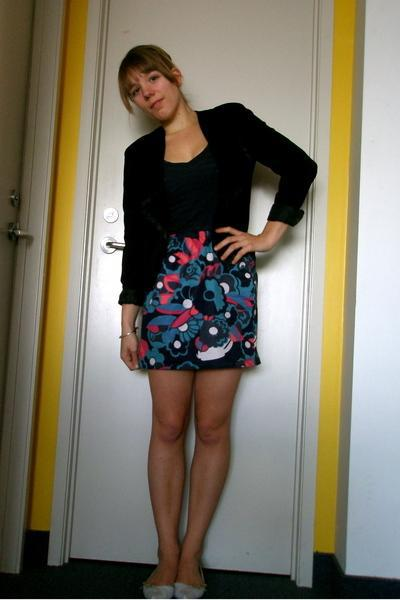
\includegraphics[width=.15\textwidth]{figures/processedimages/original/0153056.jpg} & 
		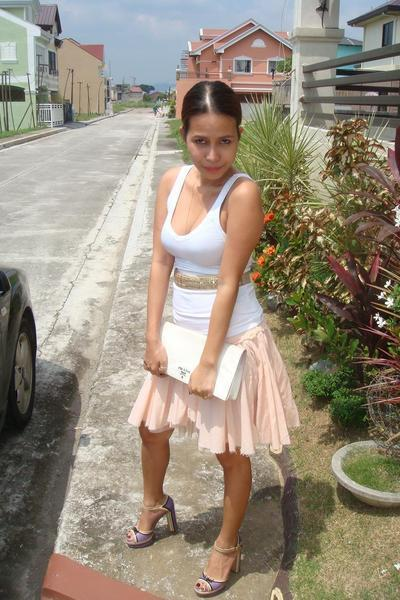
\includegraphics[width=.15\textwidth]{figures/processedimages/original/0169465.jpg} &
		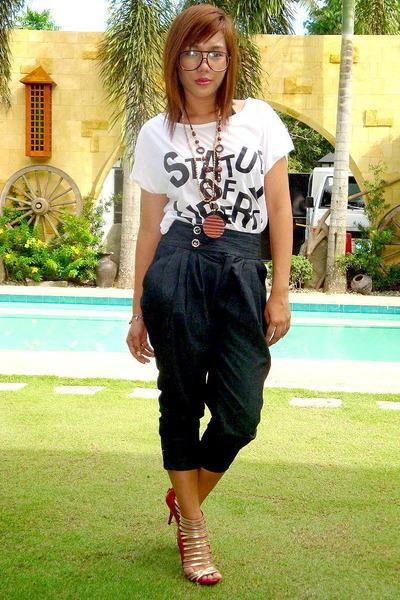
\includegraphics[width=.15\textwidth]{figures/processedimages/original/0196875.jpg} &
		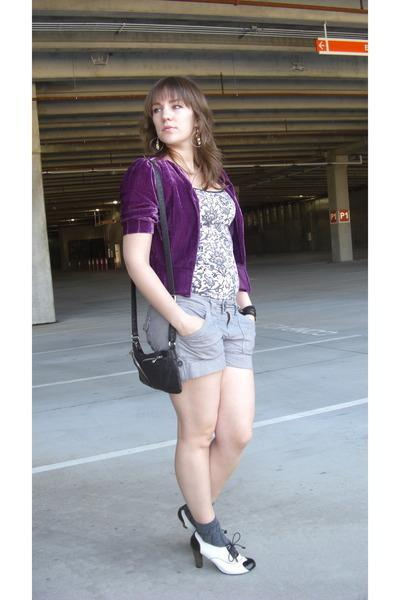
\includegraphics[width=.15\textwidth]{figures/processedimages/original/0201966.jpg} &
		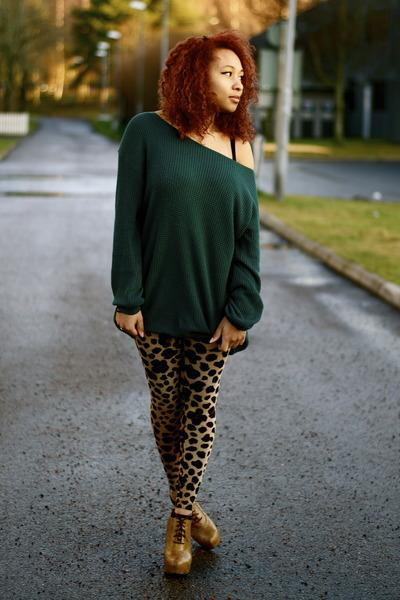
\includegraphics[width=.15\textwidth]{figures/processedimages/original/0289352.jpg} &
		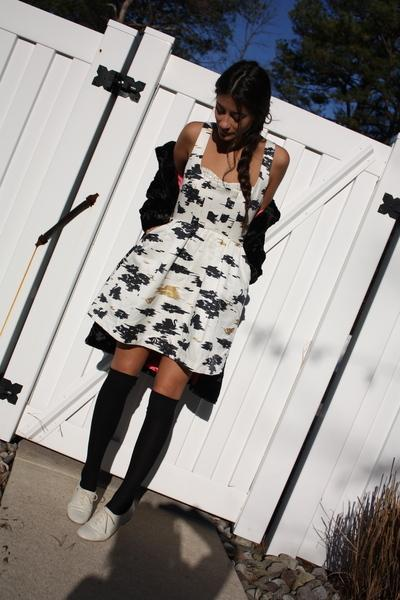
\includegraphics[width=.15\textwidth]{figures/processedimages/original/0339823.jpg}\\
		%\vspace{-5mm}
		%2nd row----------------------------
		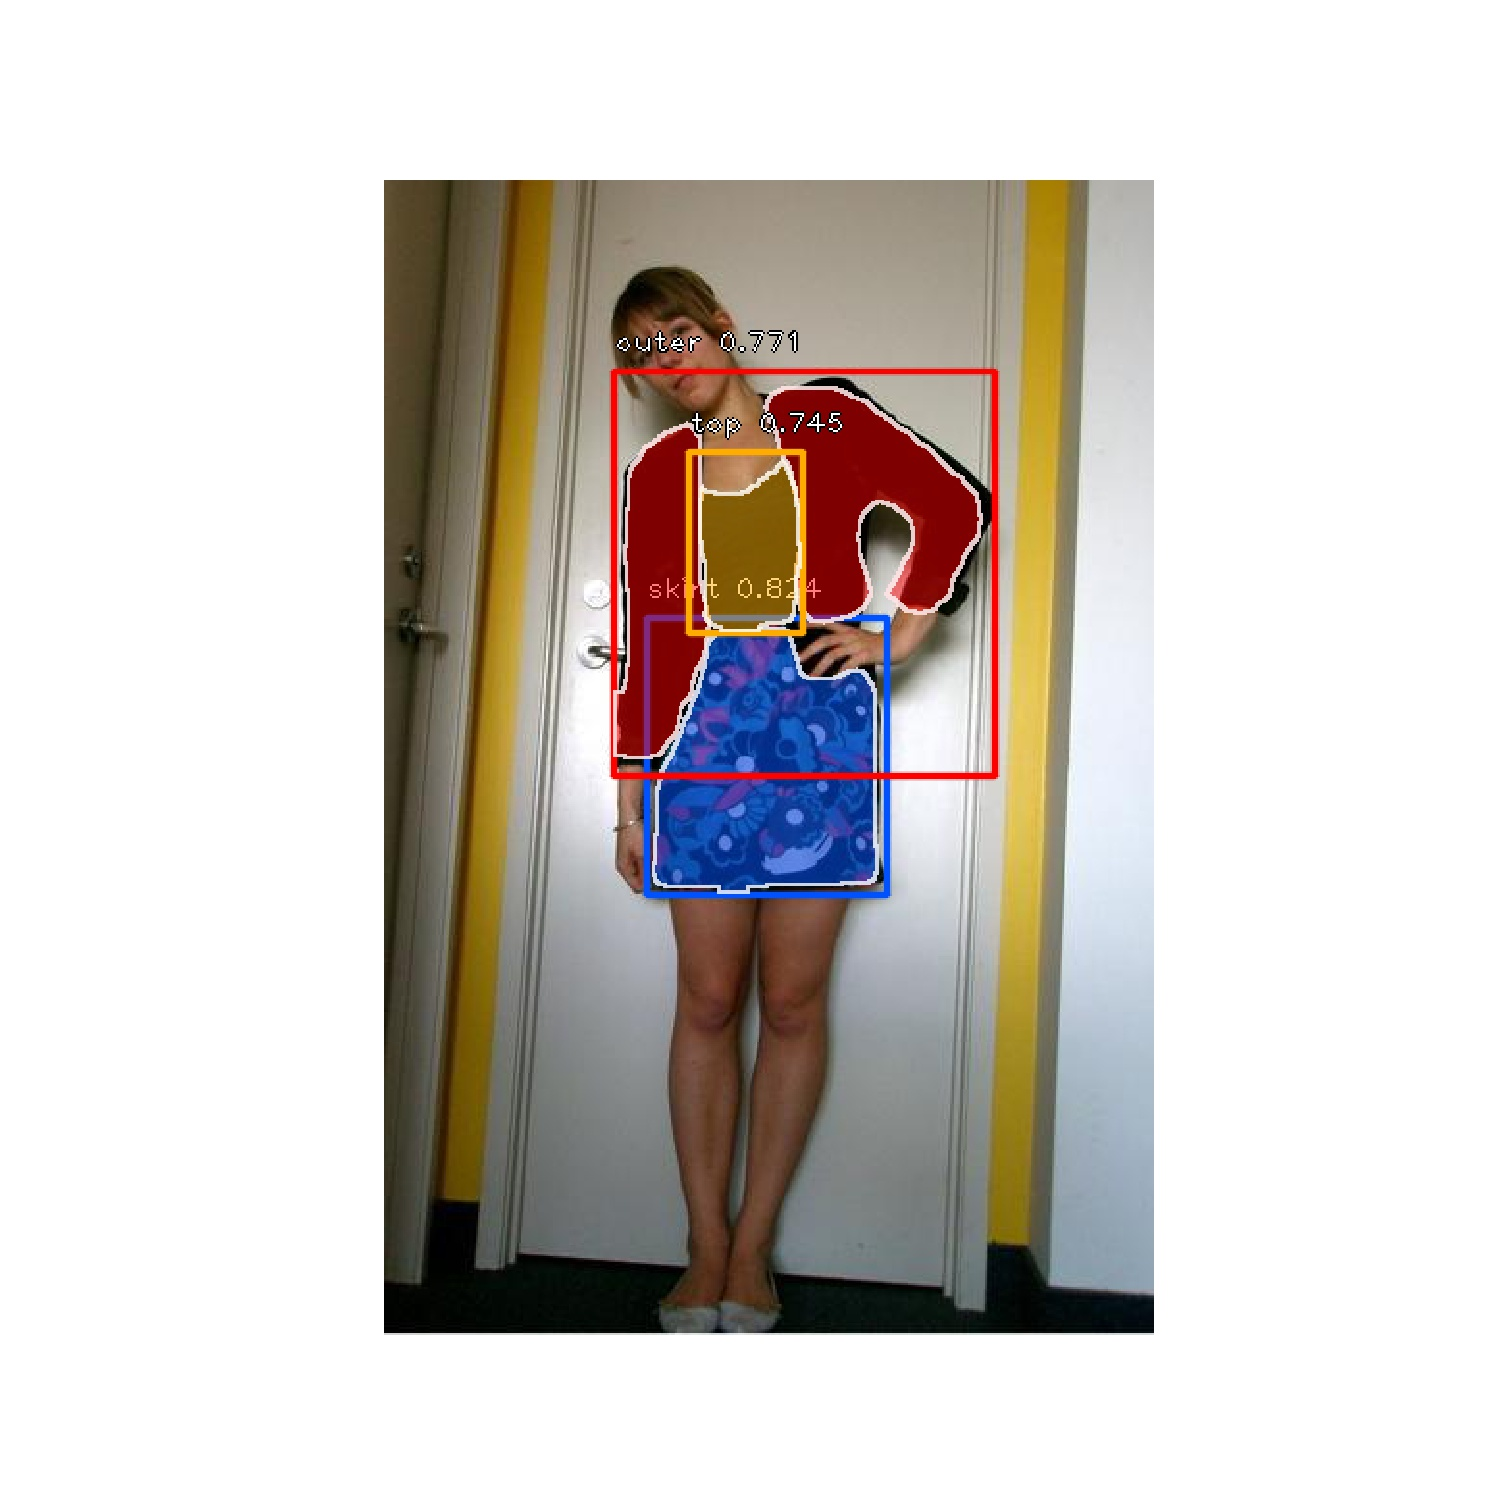
\includegraphics[width=.15\textwidth ,trim=13cm 5cm 13cm 5cm,clip]{figures/processedimages/28fixedindices/0153056} & 
		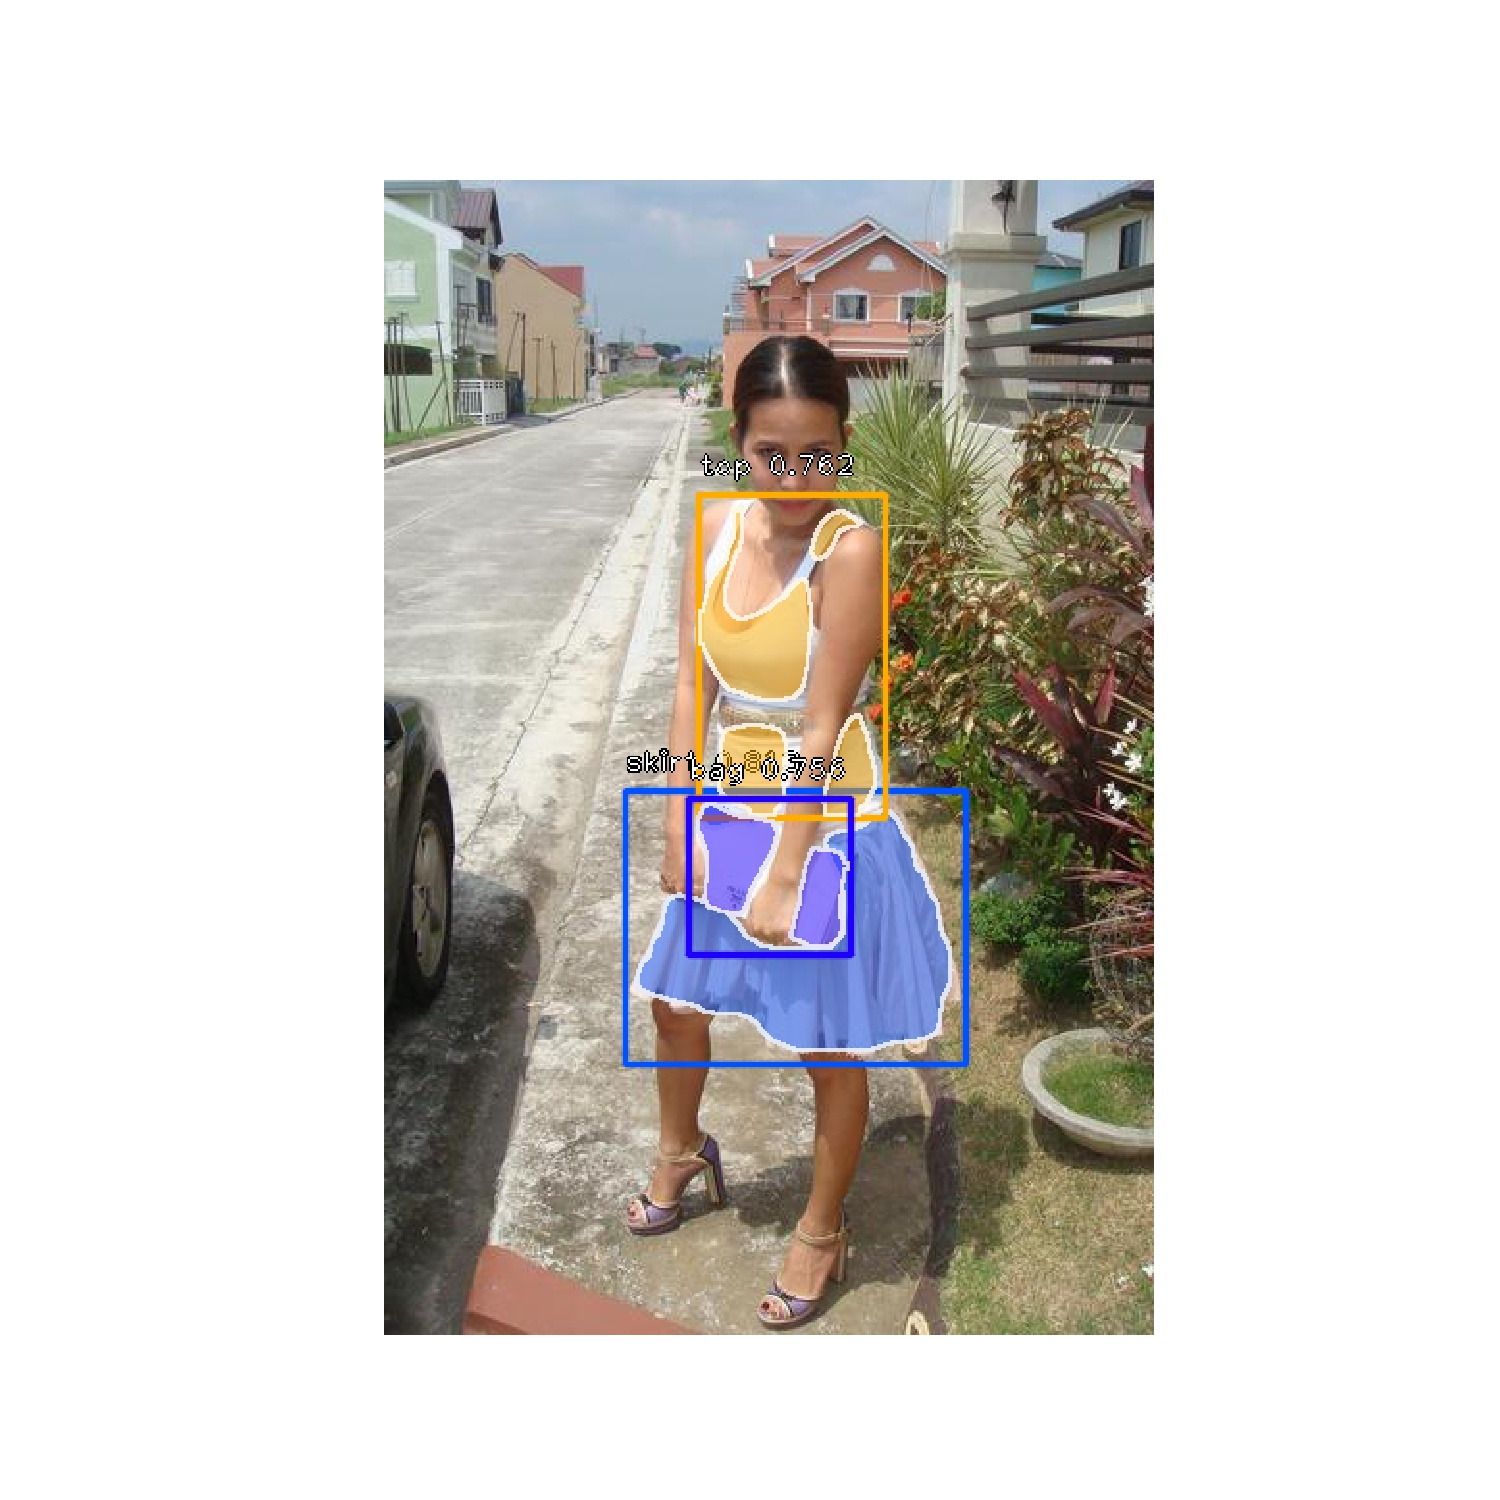
\includegraphics[width=.15\textwidth ,trim=13cm 5cm 13cm 5cm,clip]{figures/processedimages/28fixedindices/0169465} &
		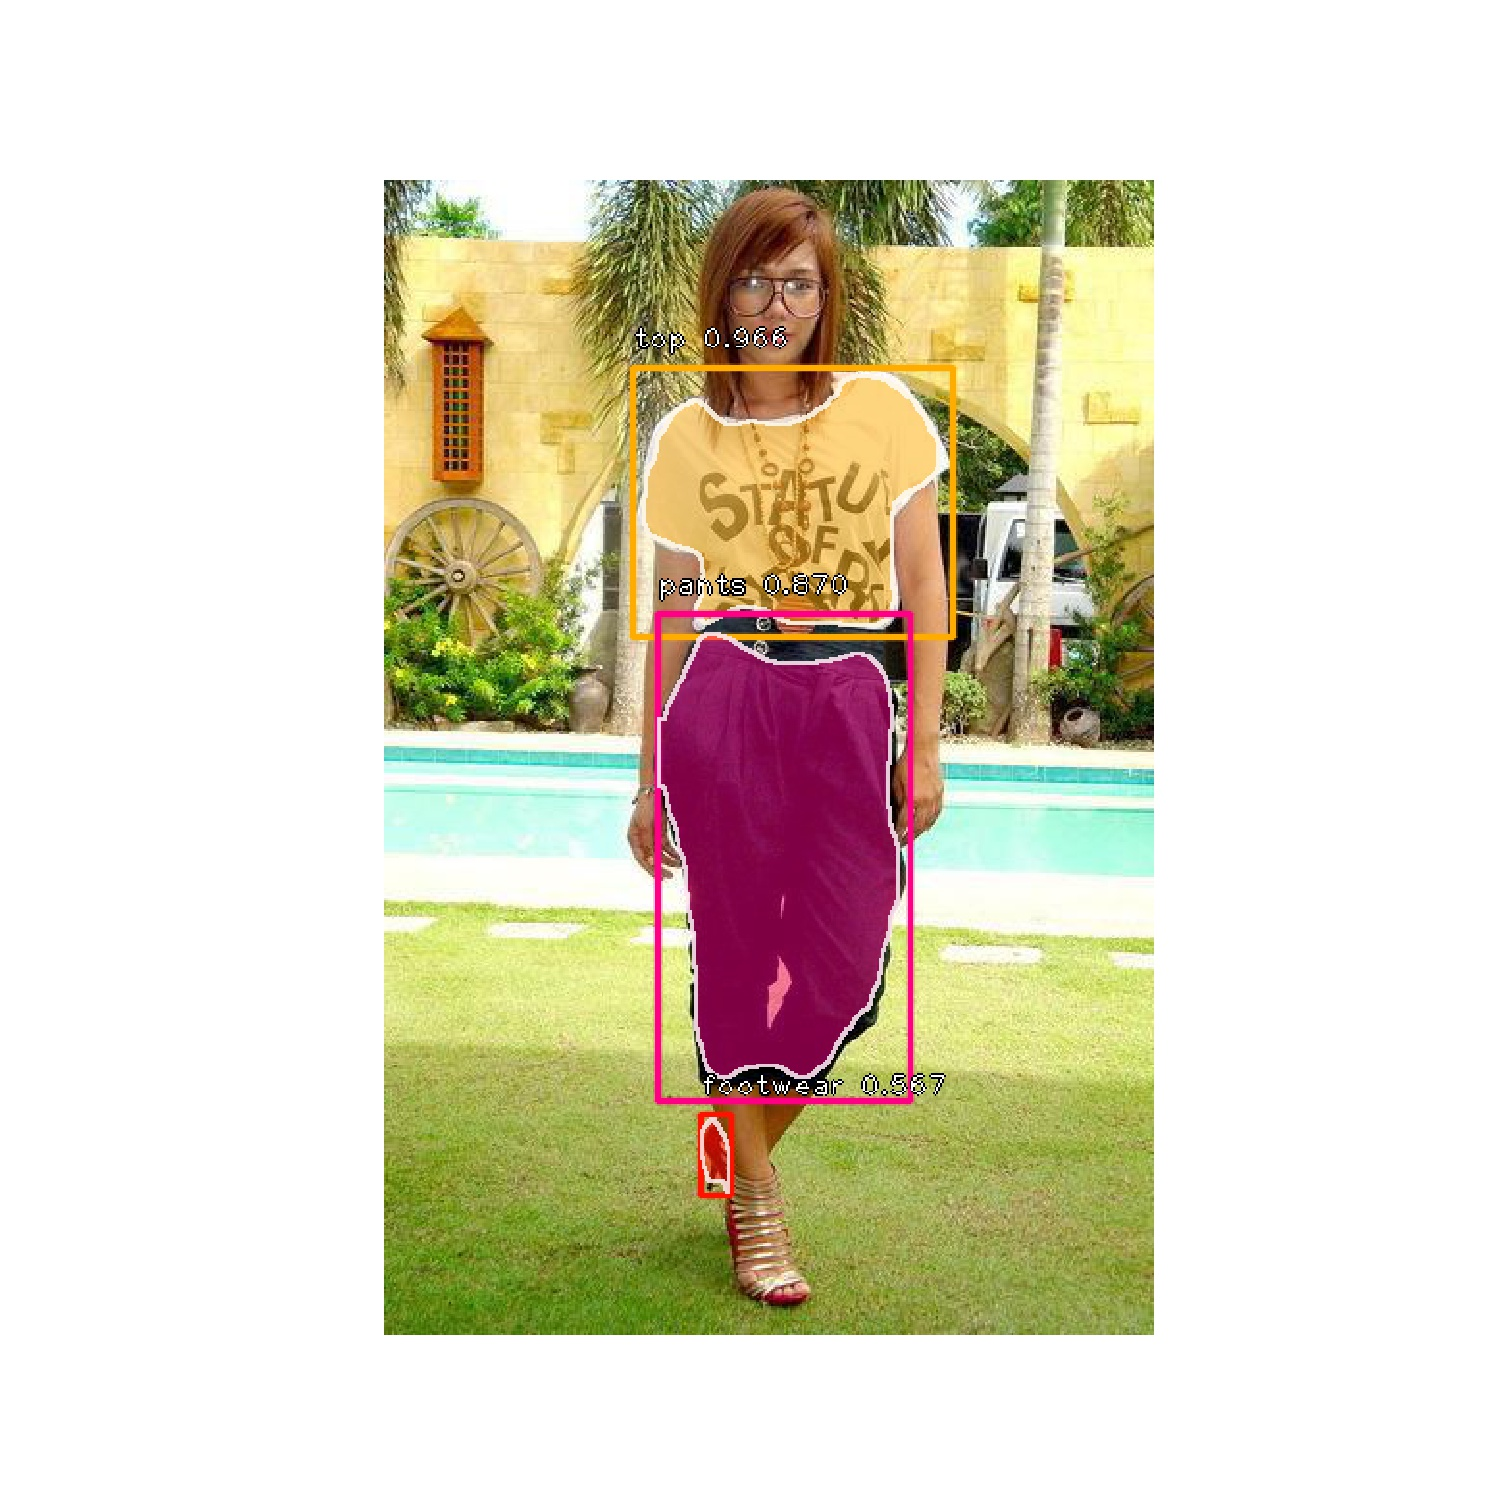
\includegraphics[width=.15\textwidth ,trim=13cm 5cm 13cm 5cm,clip]{figures/processedimages/28fixedindices/0196875} &
		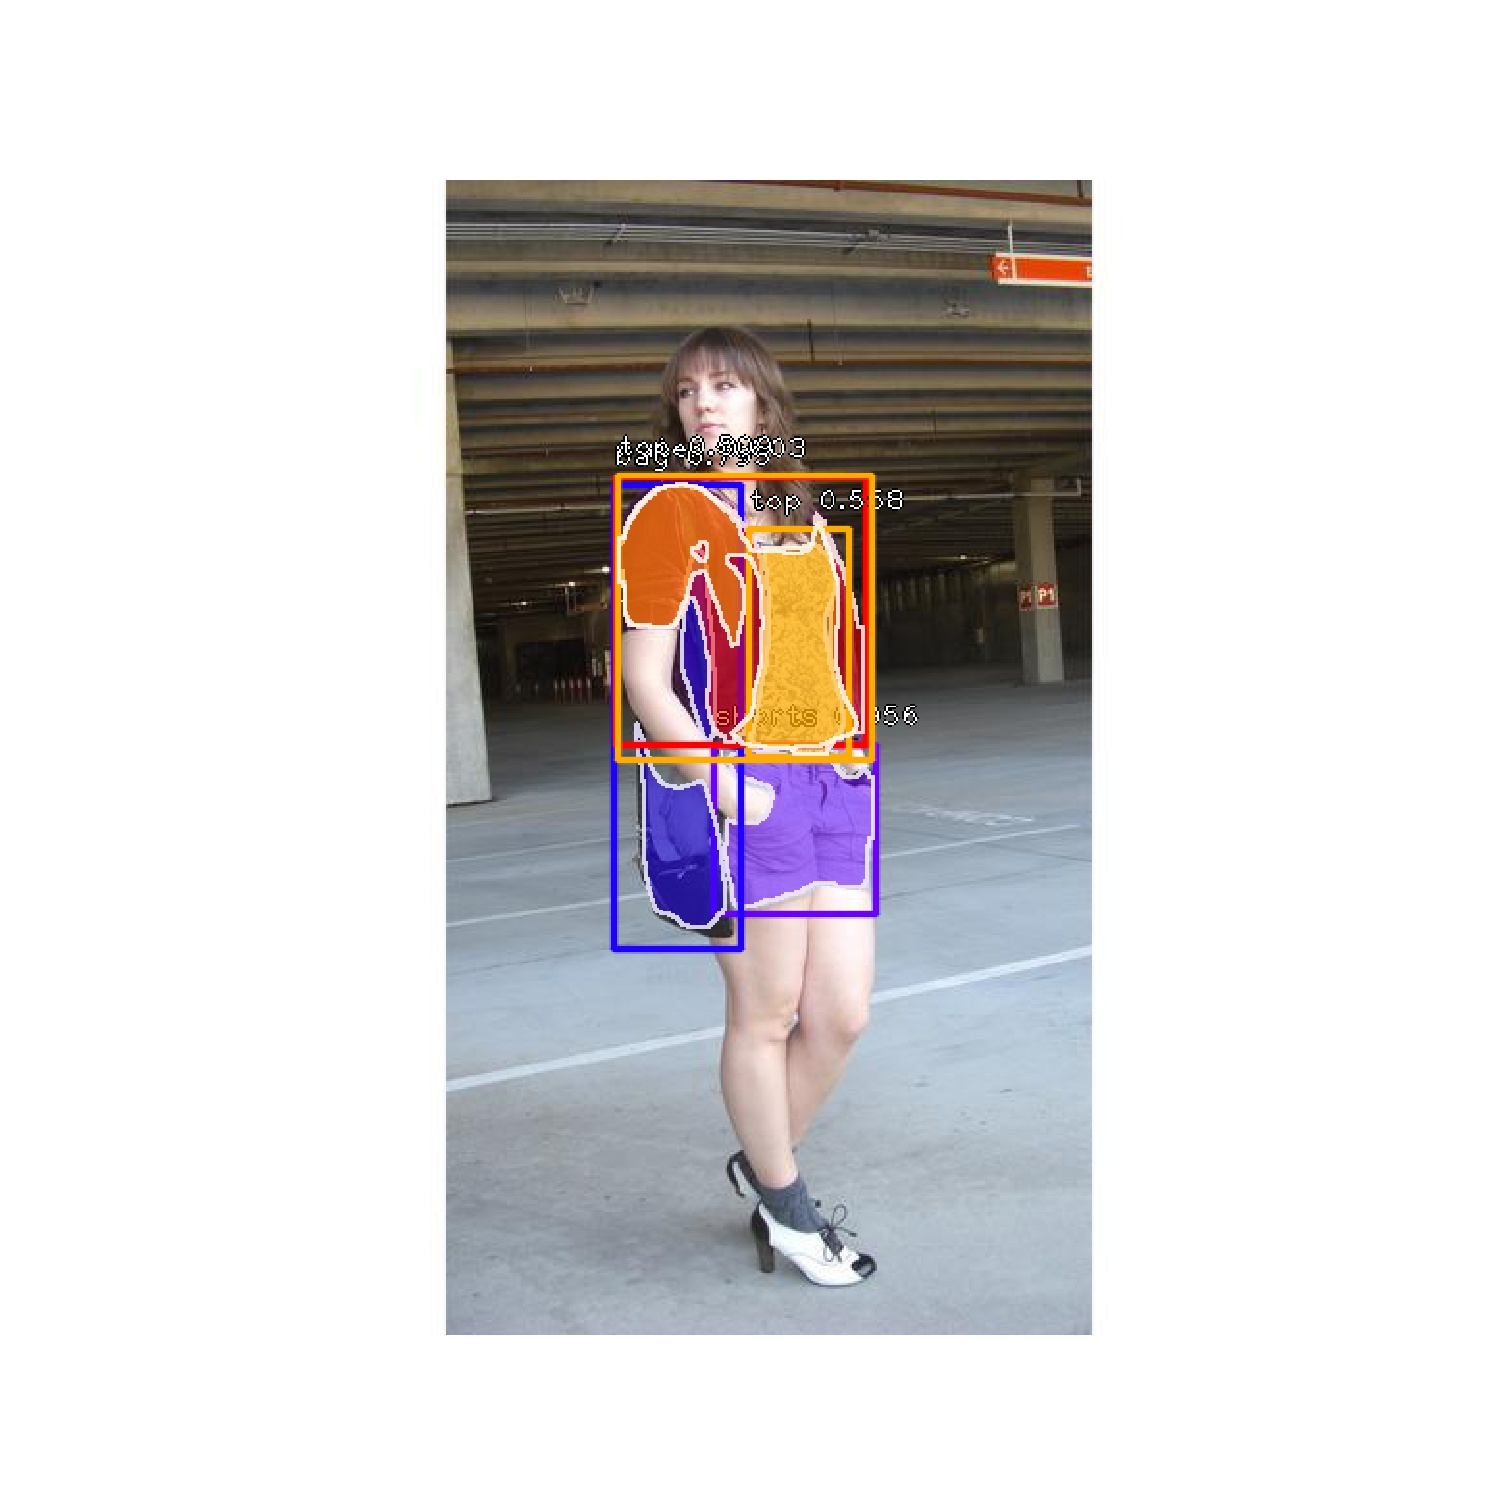
\includegraphics[width=.15\textwidth ,trim=13cm 5cm 13cm 5cm,clip]{figures/processedimages/28fixedindices/0201966} &
		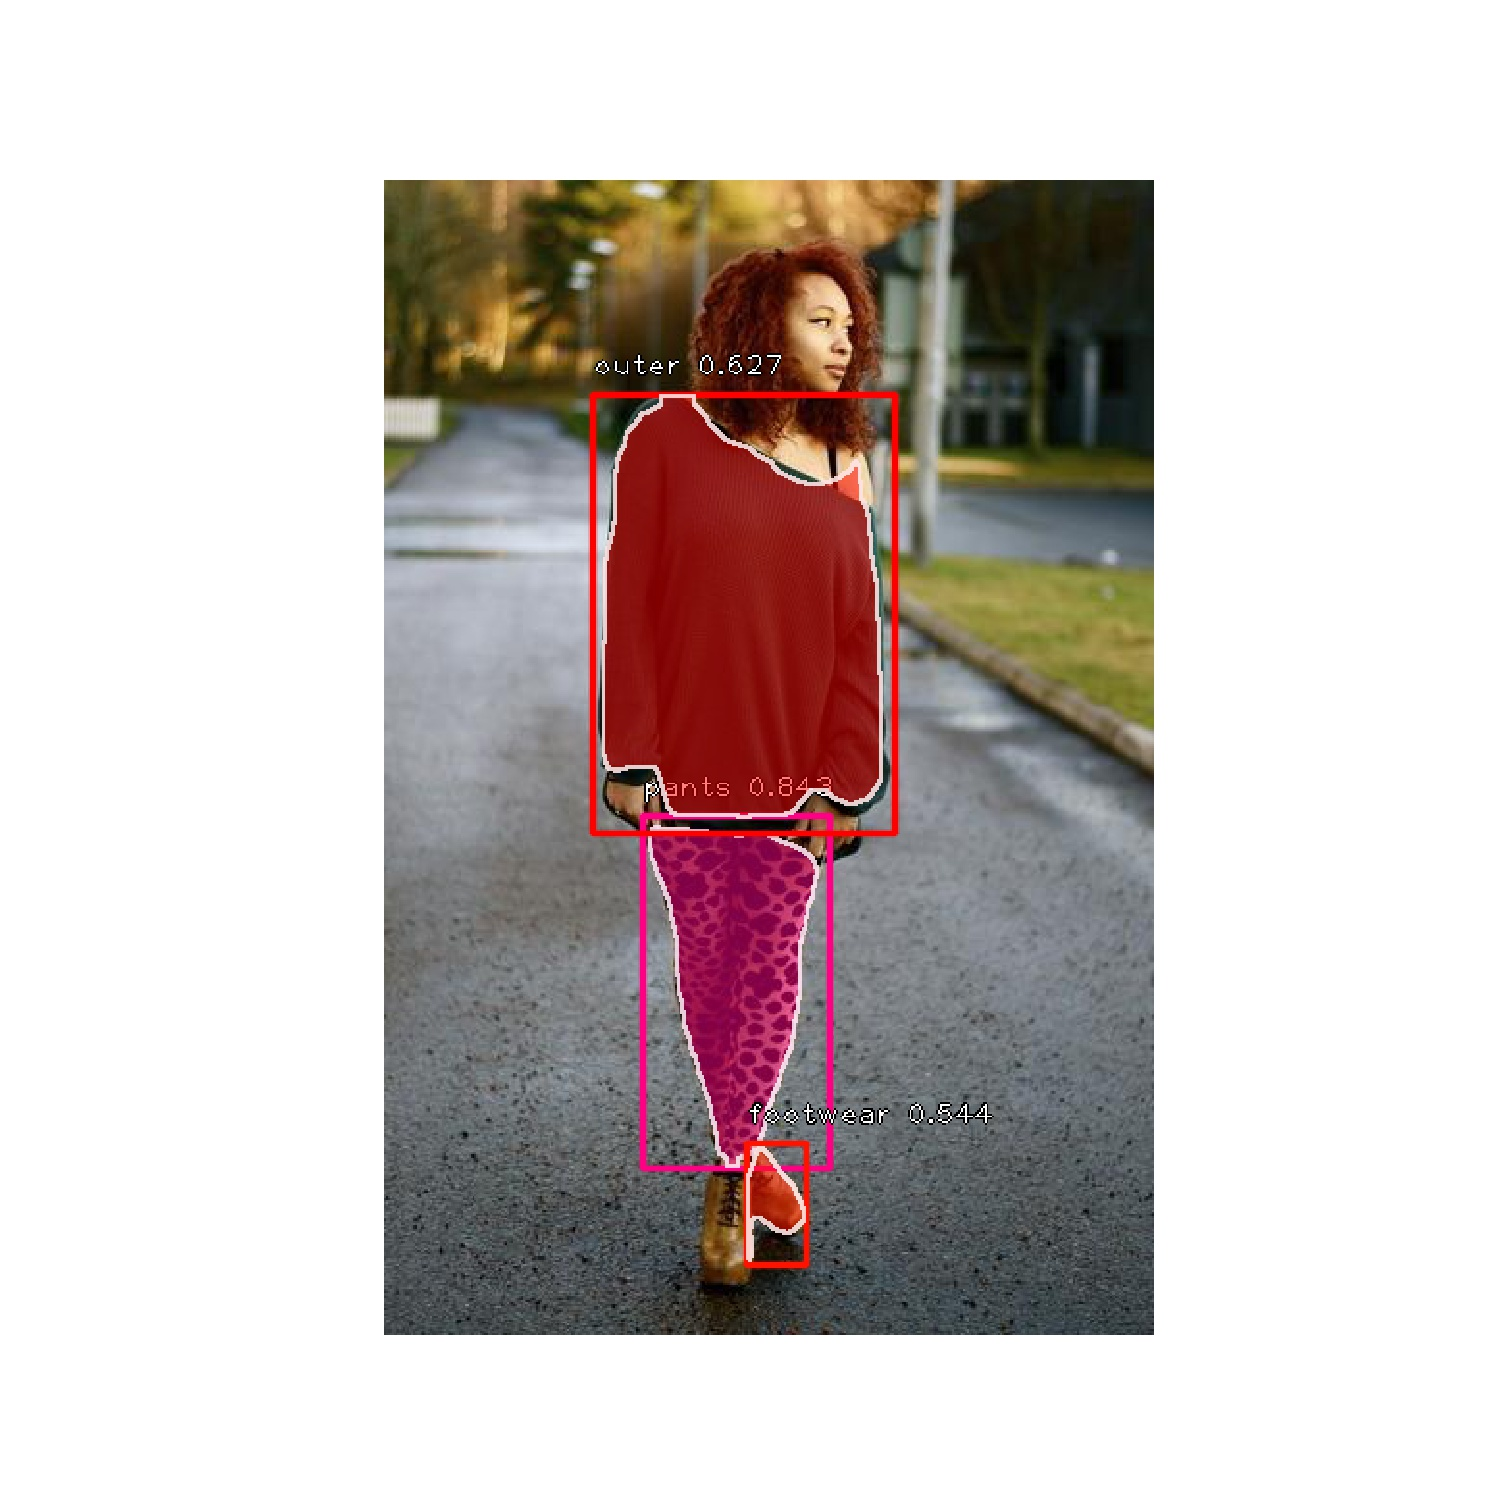
\includegraphics[width=.15\textwidth ,trim=13cm 5cm 13cm 5cm,clip]{figures/processedimages/28fixedindices/0289352} & 
		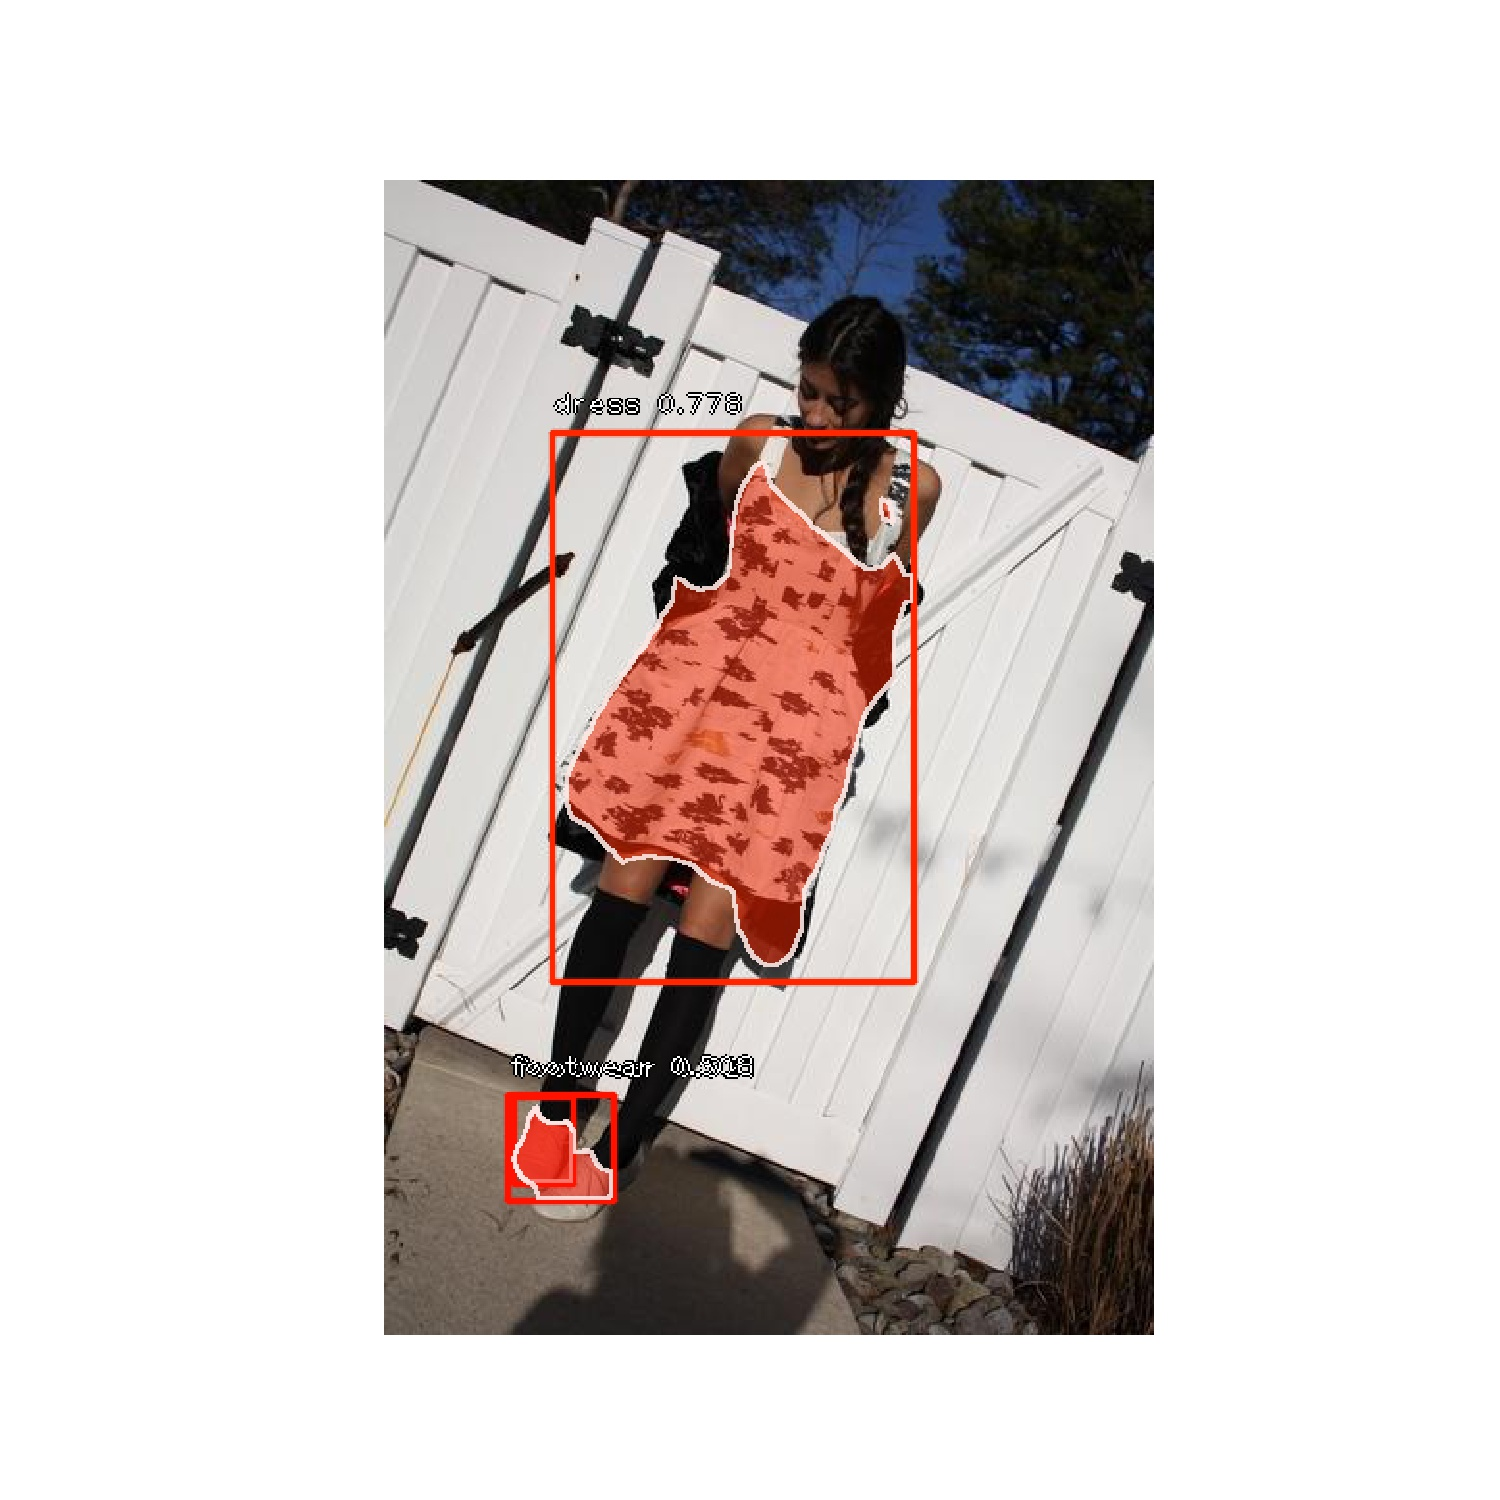
\includegraphics[width=.15\textwidth ,trim=13cm 5cm 13cm 5cm,clip]{figures/processedimages/28fixedindices/0339823}\\
		%\vspace{-5mm}
		%3rd row----------------------------
		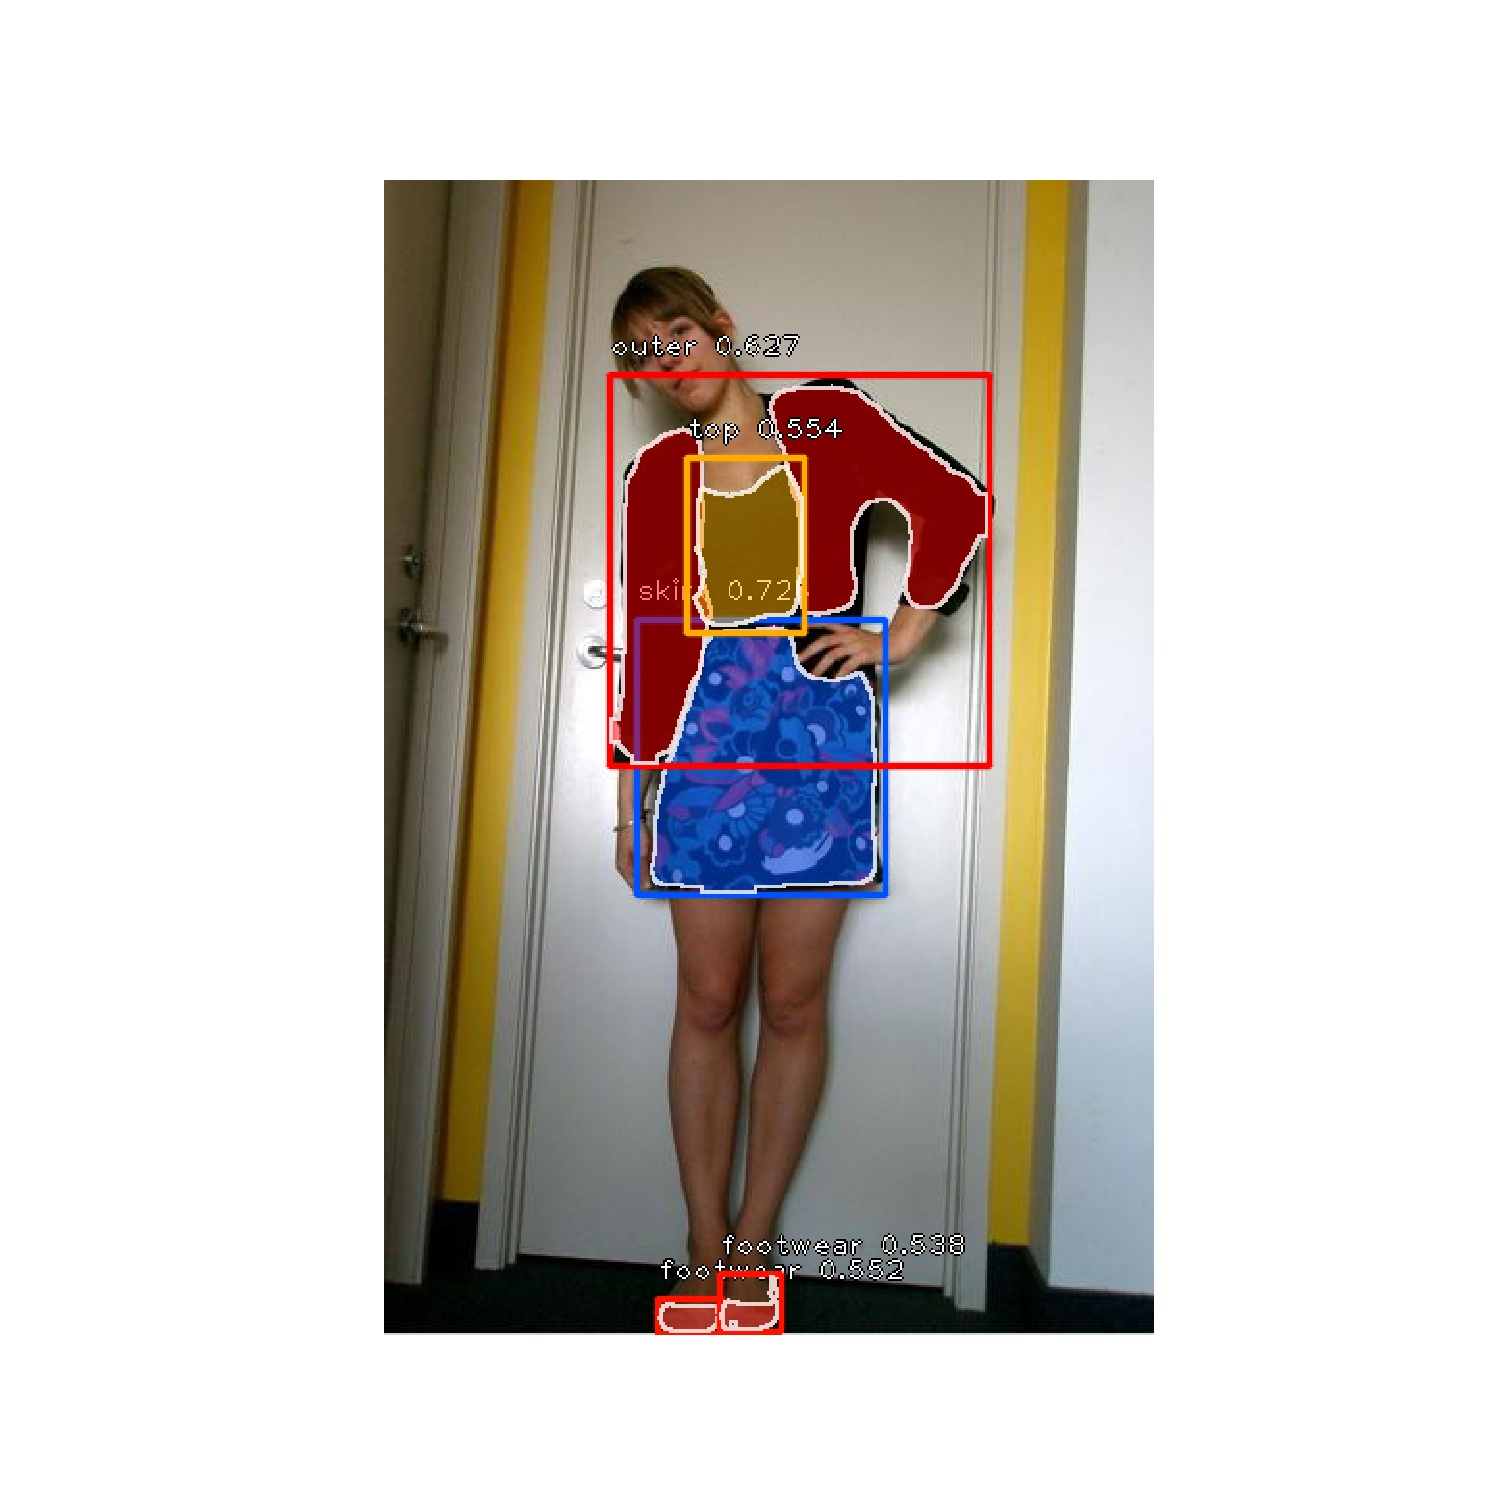
\includegraphics[width=.15\textwidth ,trim=13cm 5cm 13cm 5cm,clip]{figures/processedimages/7afteralmostnewwrongdoubleadded/0153056} & 
		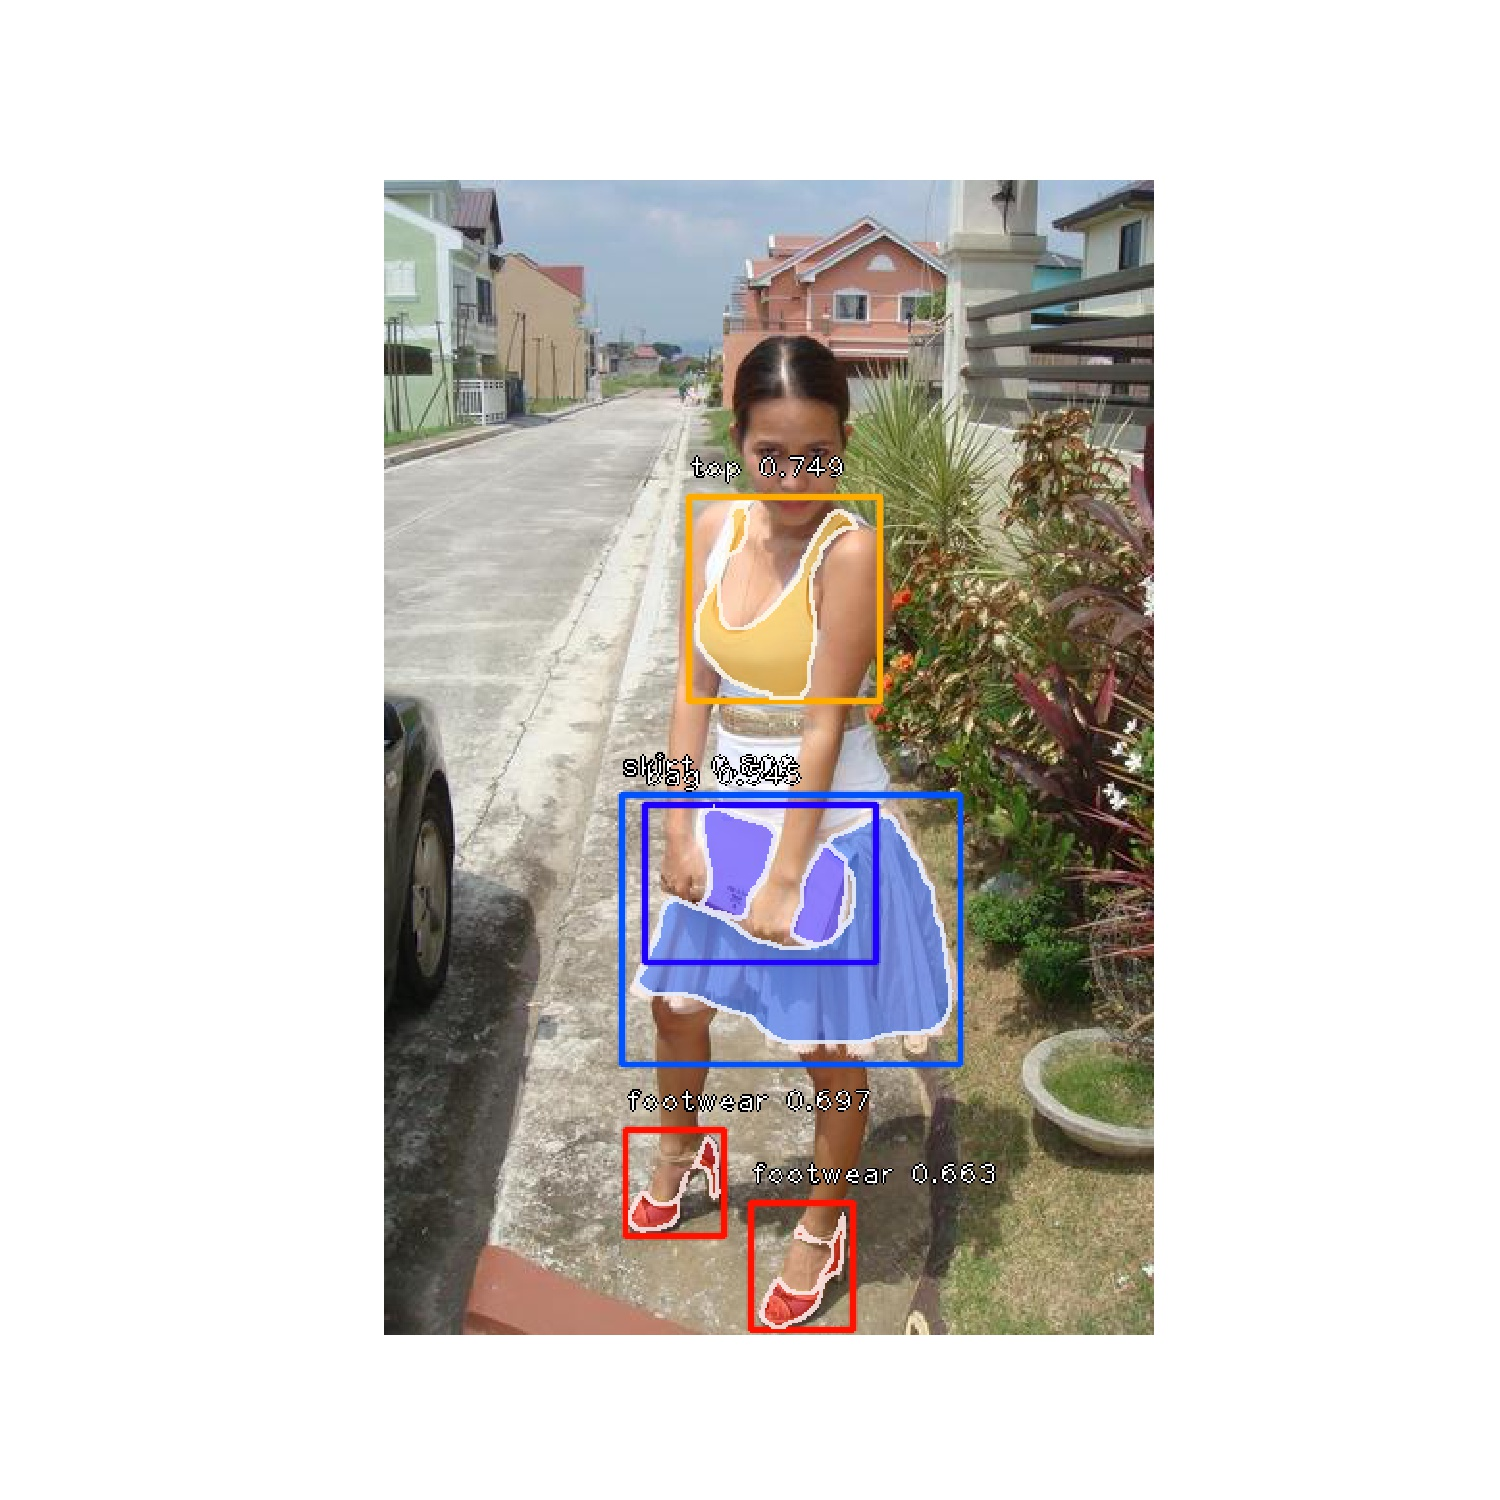
\includegraphics[width=.15\textwidth ,trim=13cm 5cm 13cm 5cm,clip]{figures/processedimages/7afteralmostnewwrongdoubleadded/0169465} &
		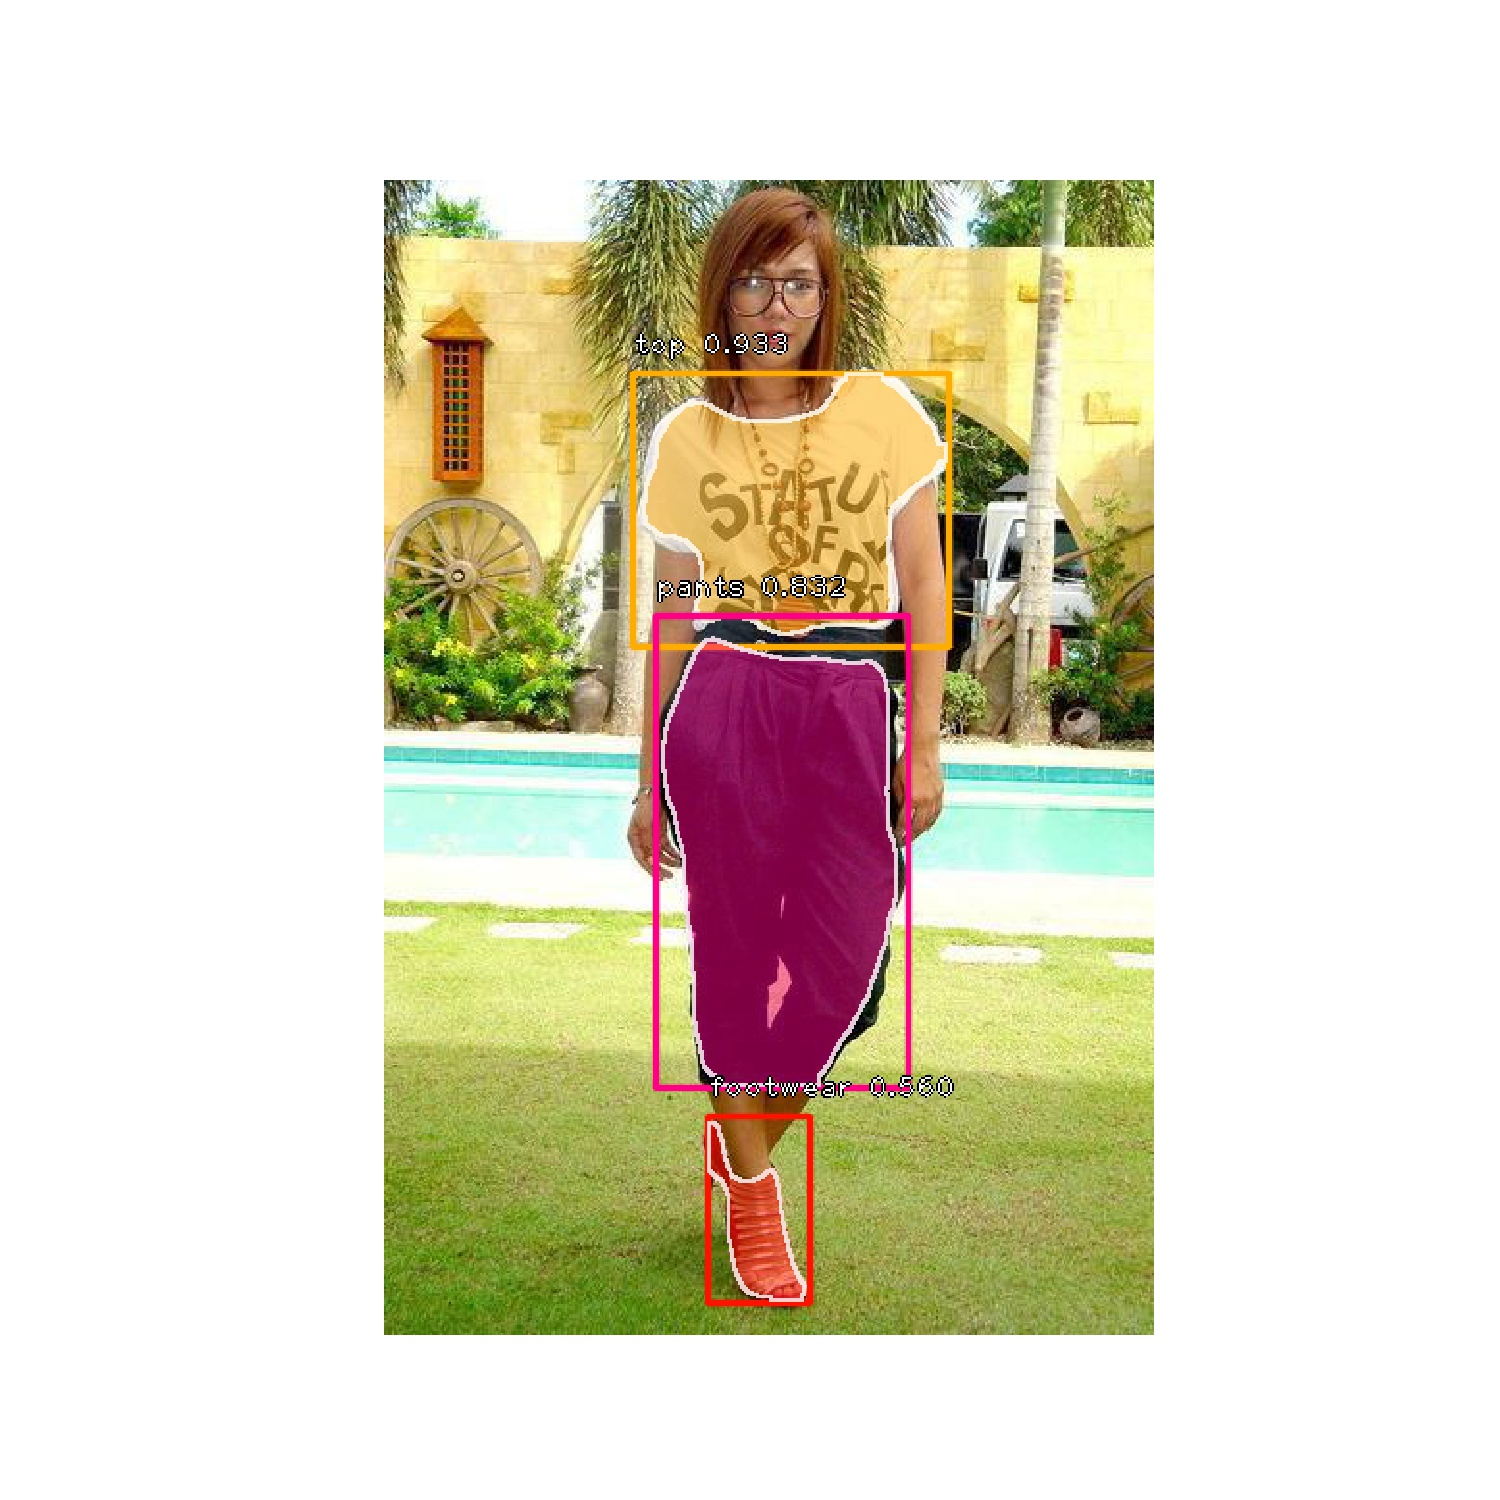
\includegraphics[width=.15\textwidth ,trim=13cm 5cm 13cm 5cm,clip]{figures/processedimages/7afteralmostnewwrongdoubleadded/0196875} &
		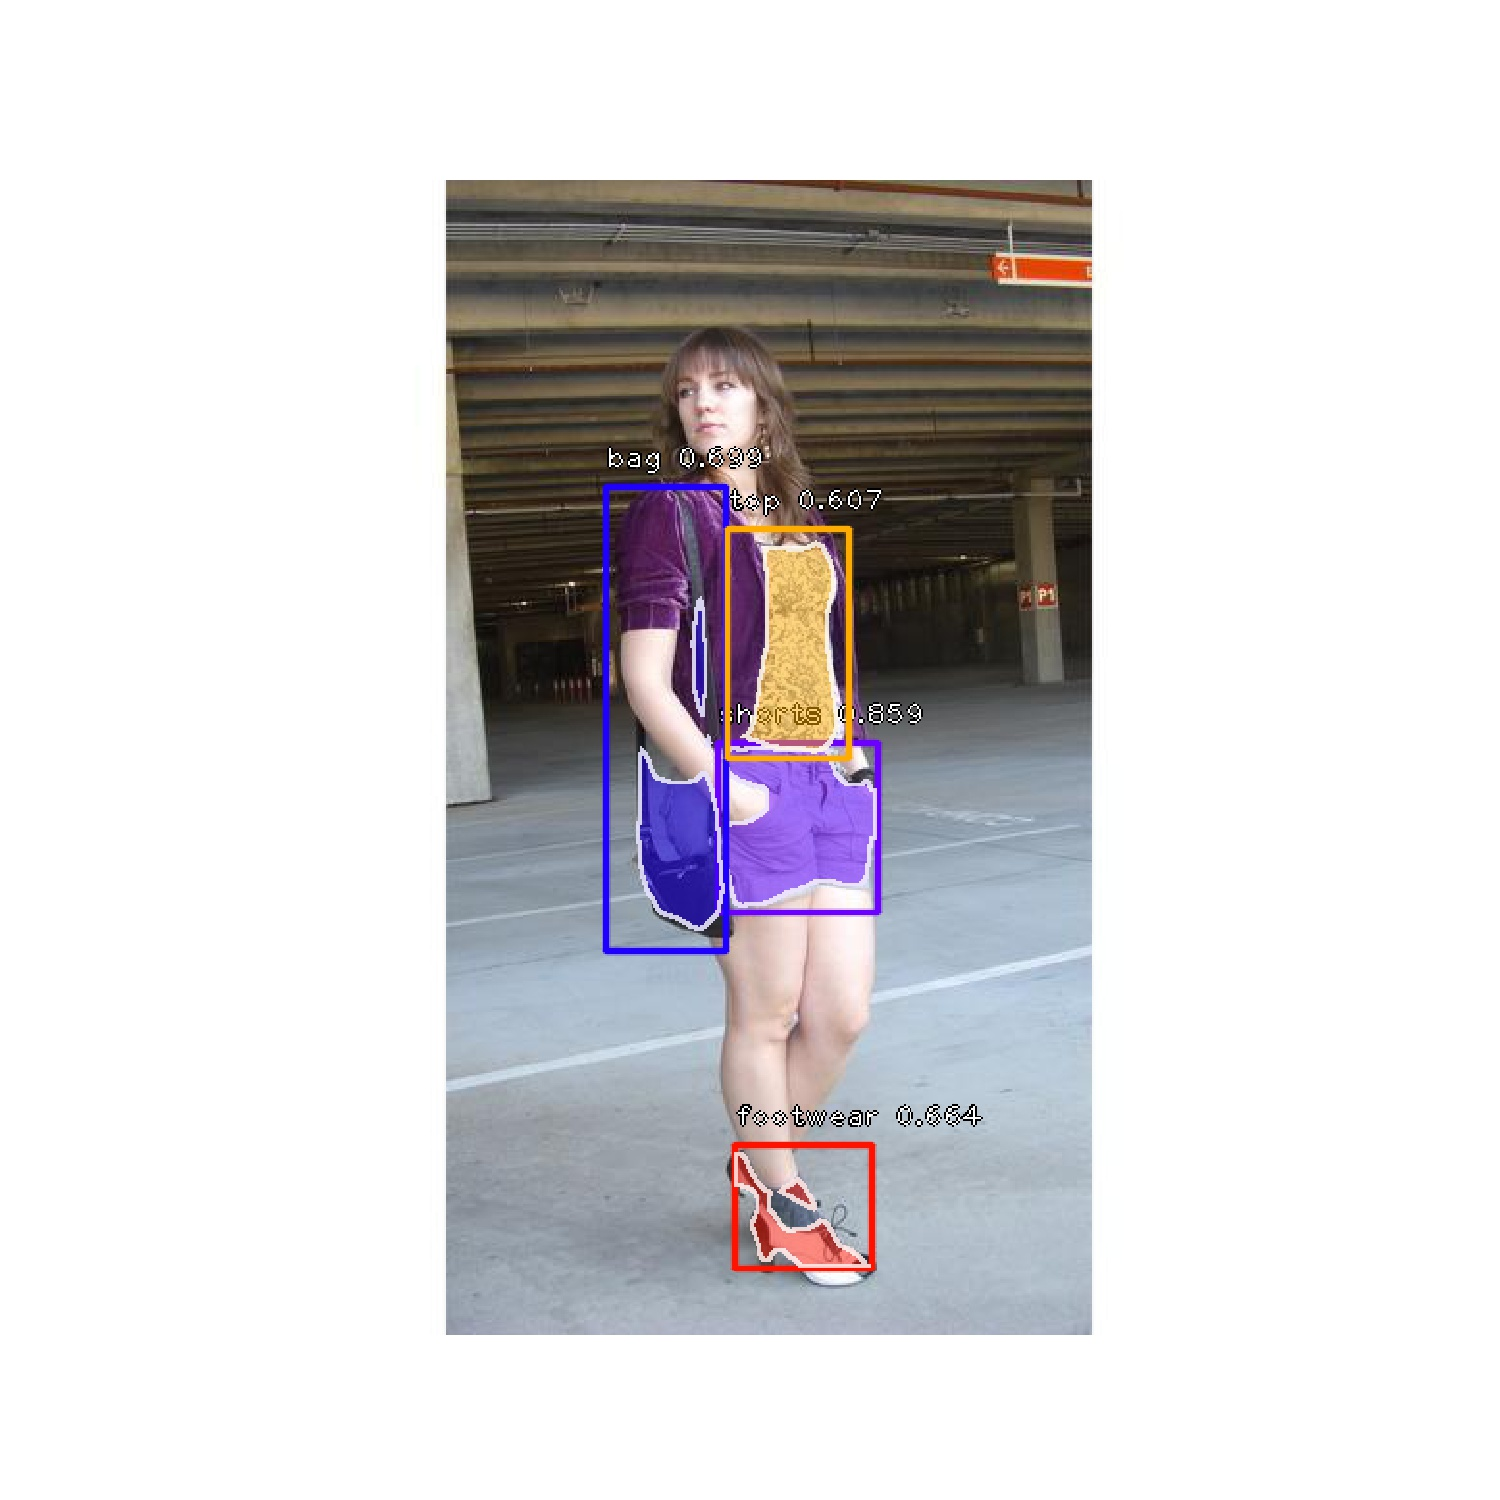
\includegraphics[width=.15\textwidth ,trim=13cm 5cm 13cm 5cm,clip]{figures/processedimages/7afteralmostnewwrongdoubleadded/0201966} &
		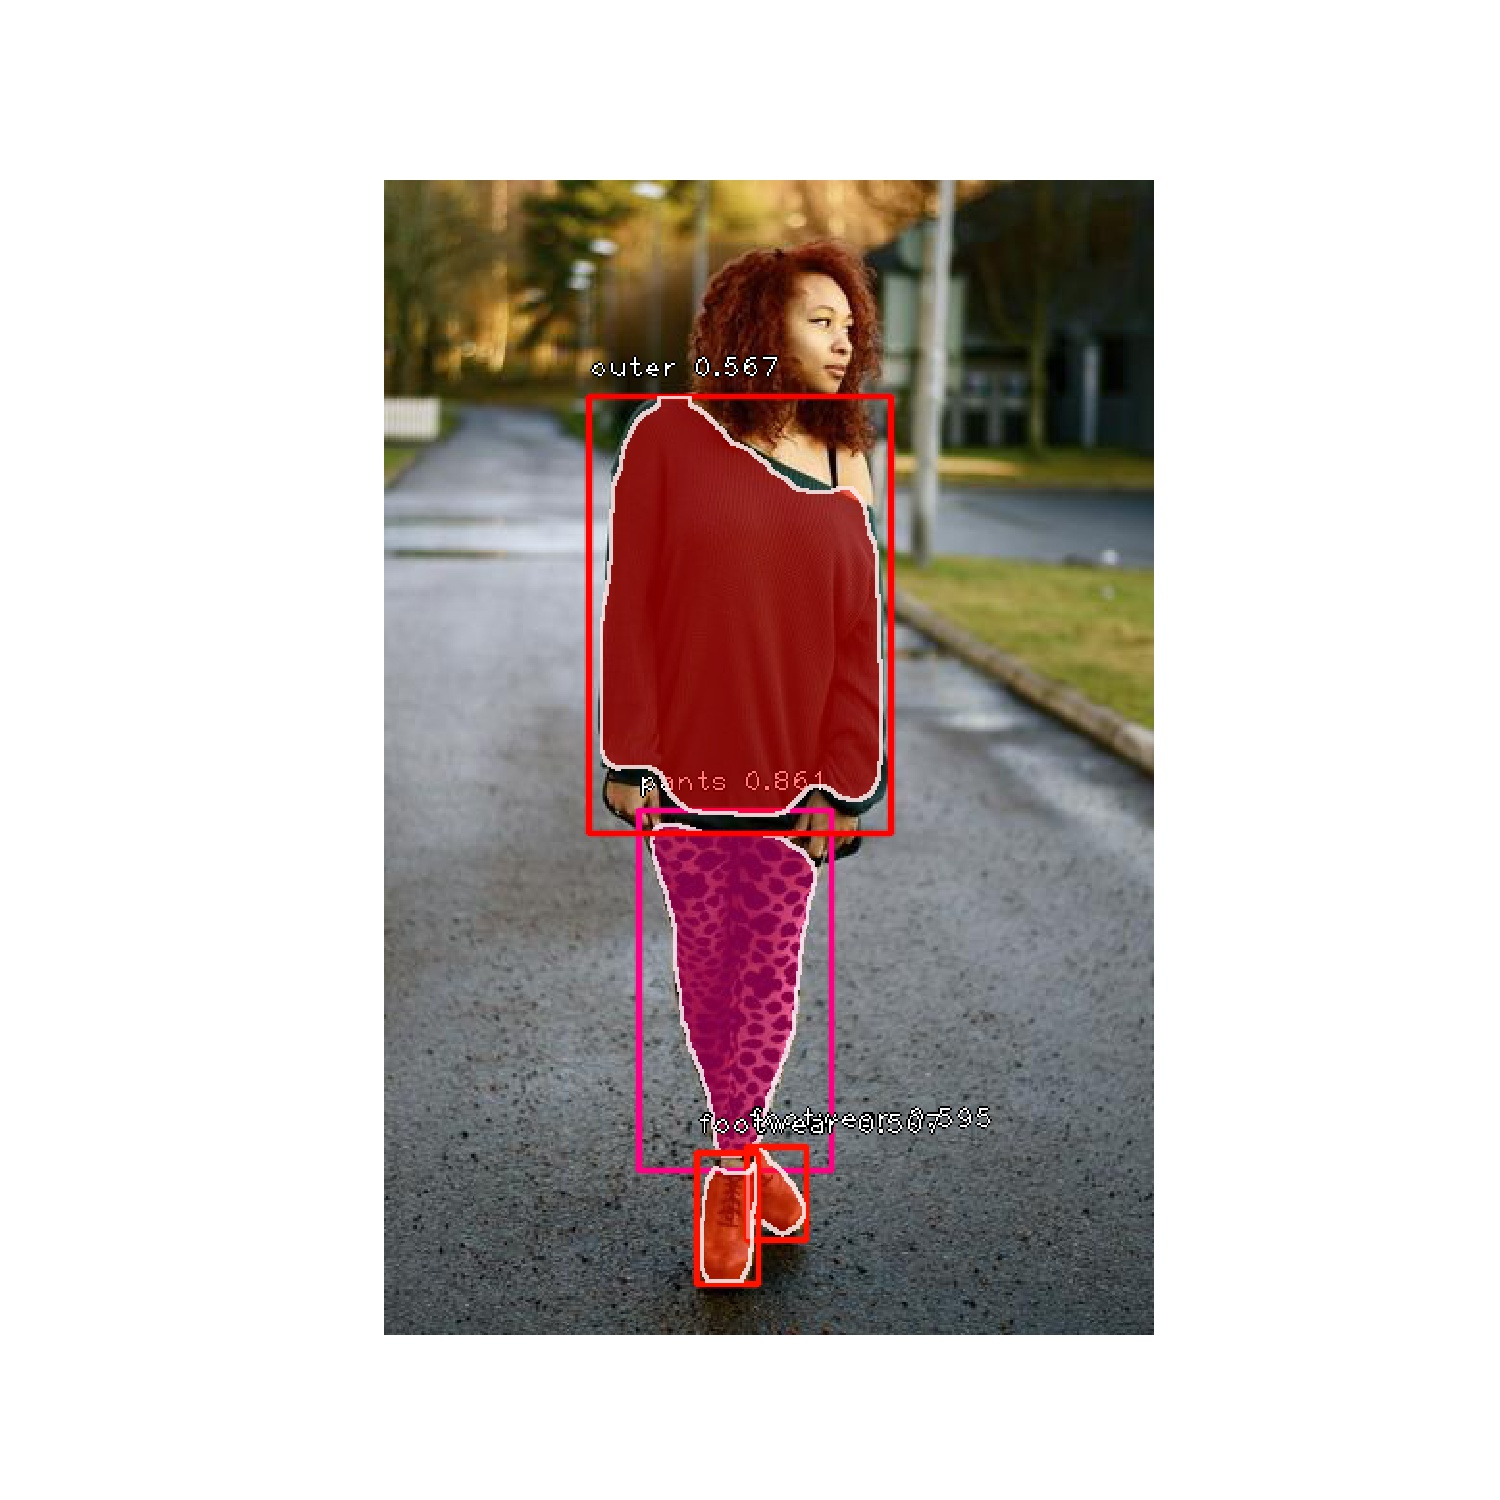
\includegraphics[width=.15\textwidth ,trim=13cm 5cm 13cm 5cm,clip]{figures/processedimages/7afteralmostnewwrongdoubleadded/0289352} & 
		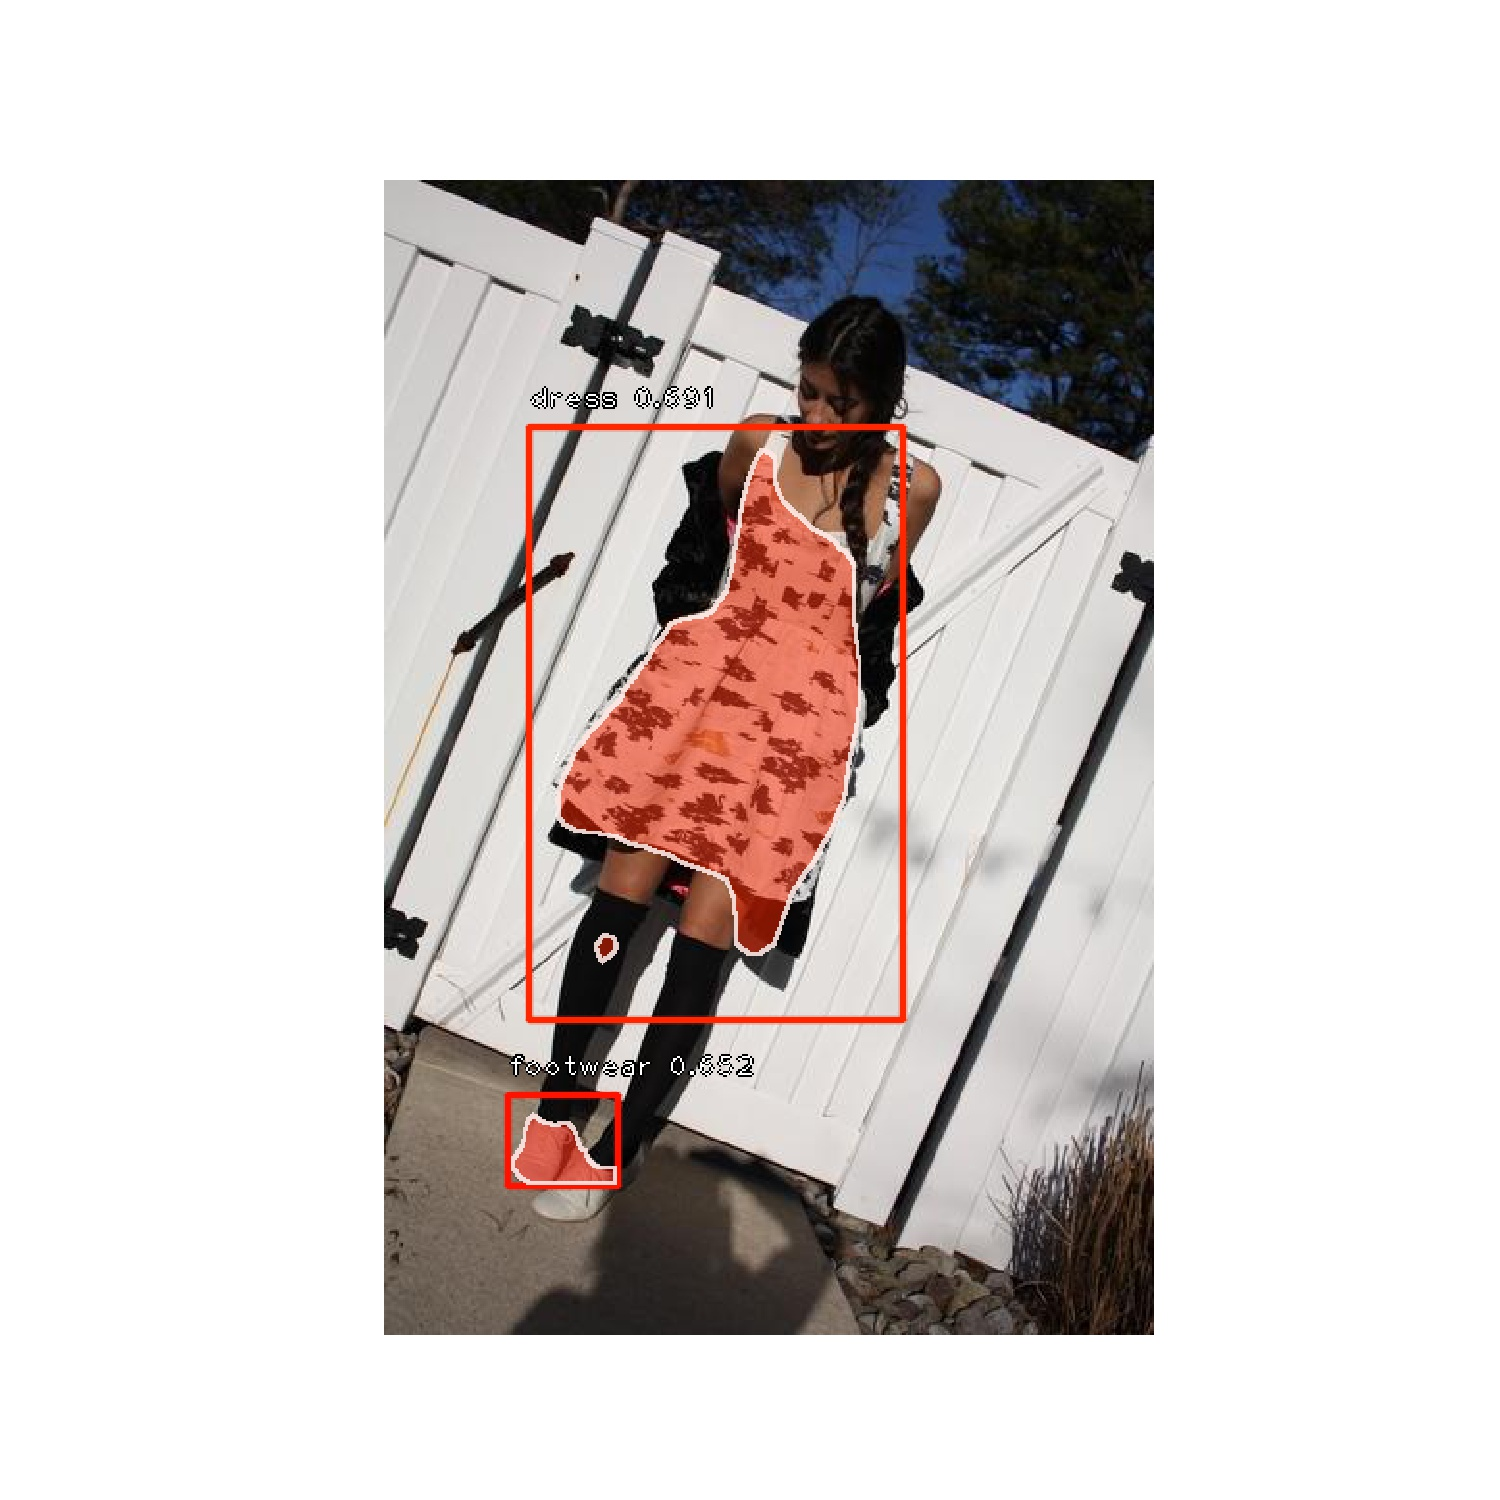
\includegraphics[width=.15\textwidth ,trim=13cm 5cm 13cm 5cm,clip]{figures/processedimages/7afteralmostnewwrongdoubleadded/0339823}\\
		
	\end{tabular}
	\caption{Examples of original images with corresponding pixel-level segmentation masks and bounding box annotations of the proposed ModaNet dataset inferred from training. The first row shows the original color street image containing a person with fashion products. The second row shows the result of the 28 invalid indexes model, described in the previous chapter. The third row shows the new annotations' results.}
	\label{f:processedimages} %% label for entire figure
\end{figure}
% --- figure ends --- % 

And here are some examples. We selected 12 images randomly and show them for some tests. I downloaded a total of 2000 images for each model results, using a function called processimage and described below, in \sref{s:processimage}.


% --- figure begins ---%
\begin{figure}[H]
	\centering
	\setlength{\tabcolsep}{0.1pt}
	\setlength{\fboxsep}{0pt}%
	\setlength{\fboxrule}{0.1pt}%
	\renewcommand{\arraystretch}{0.6}
	\begin{tabular}{cccccc}
		%\multicolumn{1}{c}{Query} & &\multicolumn{5}{c}{Retrieved Images} & &\multicolumn{1}{c}{Query}  & &\multicolumn{5}{c}{Retrieved Images} & &\multicolumn{1}{c}{Query}  & &\multicolumn{5}{c}{Retrieved Images}\\ 
		%1st row----------------------------
		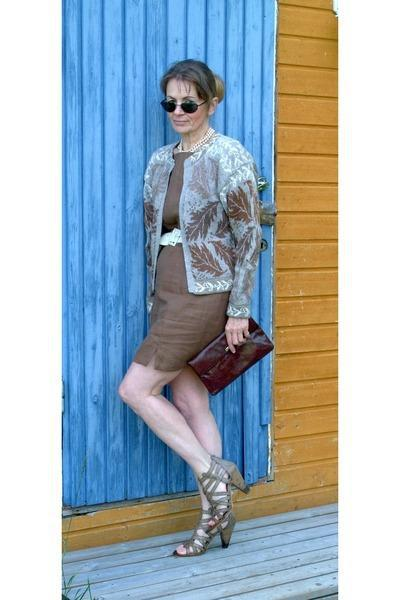
\includegraphics[width=.15\textwidth]{figures/processedimages/original/0371919.jpg} & 
		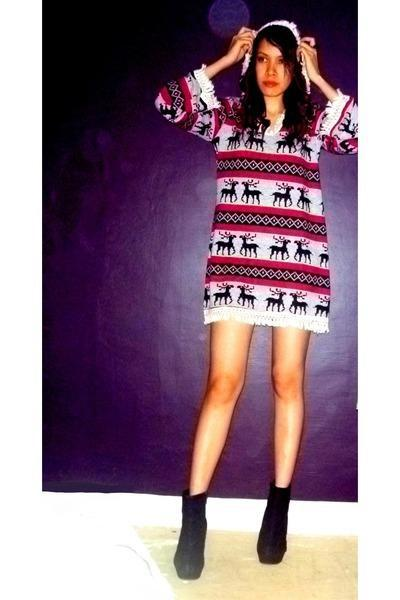
\includegraphics[width=.15\textwidth]{figures/processedimages/original/0811966.jpg} &
		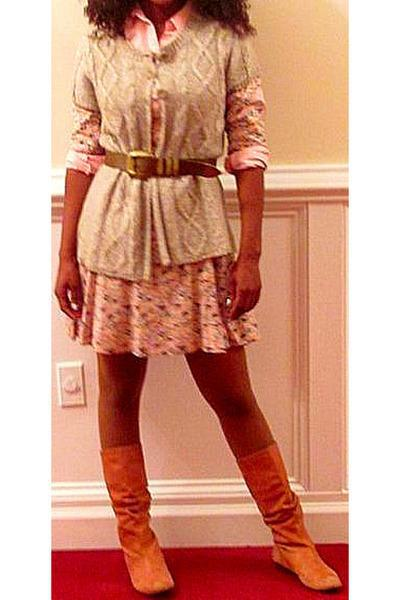
\includegraphics[width=.15\textwidth]{figures/processedimages/original/0895548.jpg} &
		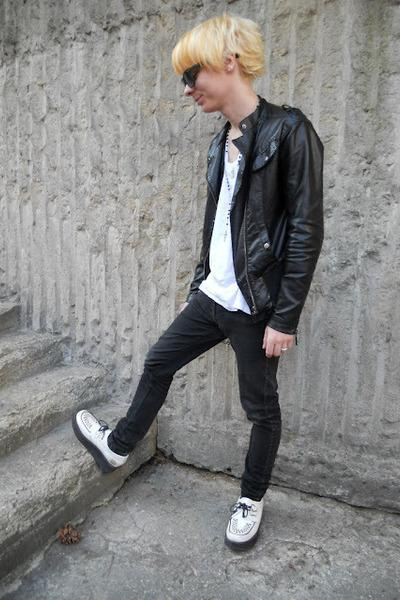
\includegraphics[width=.15\textwidth]{figures/processedimages/original/1069129.jpg} &
		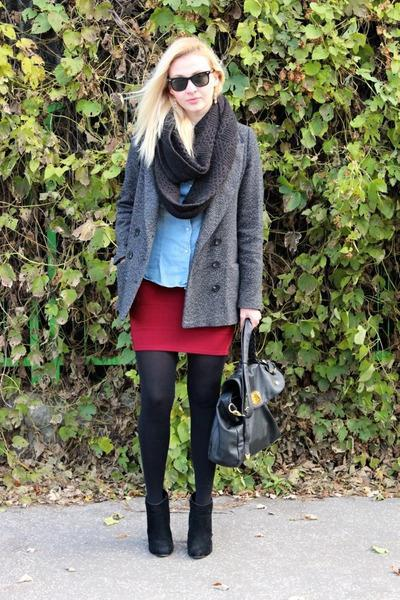
\includegraphics[width=.15\textwidth]{figures/processedimages/original/1088975.jpg} &
		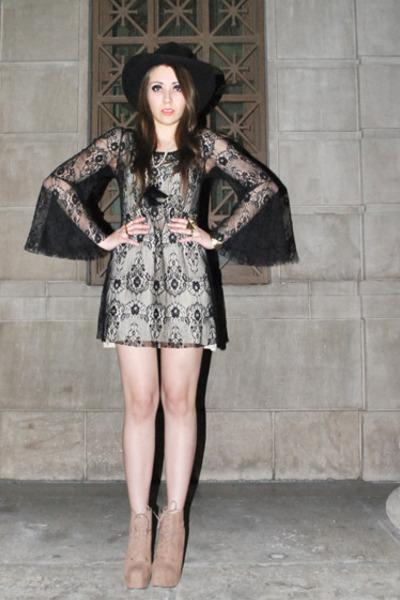
\includegraphics[width=.15\textwidth]{figures/processedimages/original/1103207.jpg}\\
		%\vspace{-5mm}
		%2nd row----------------------------
		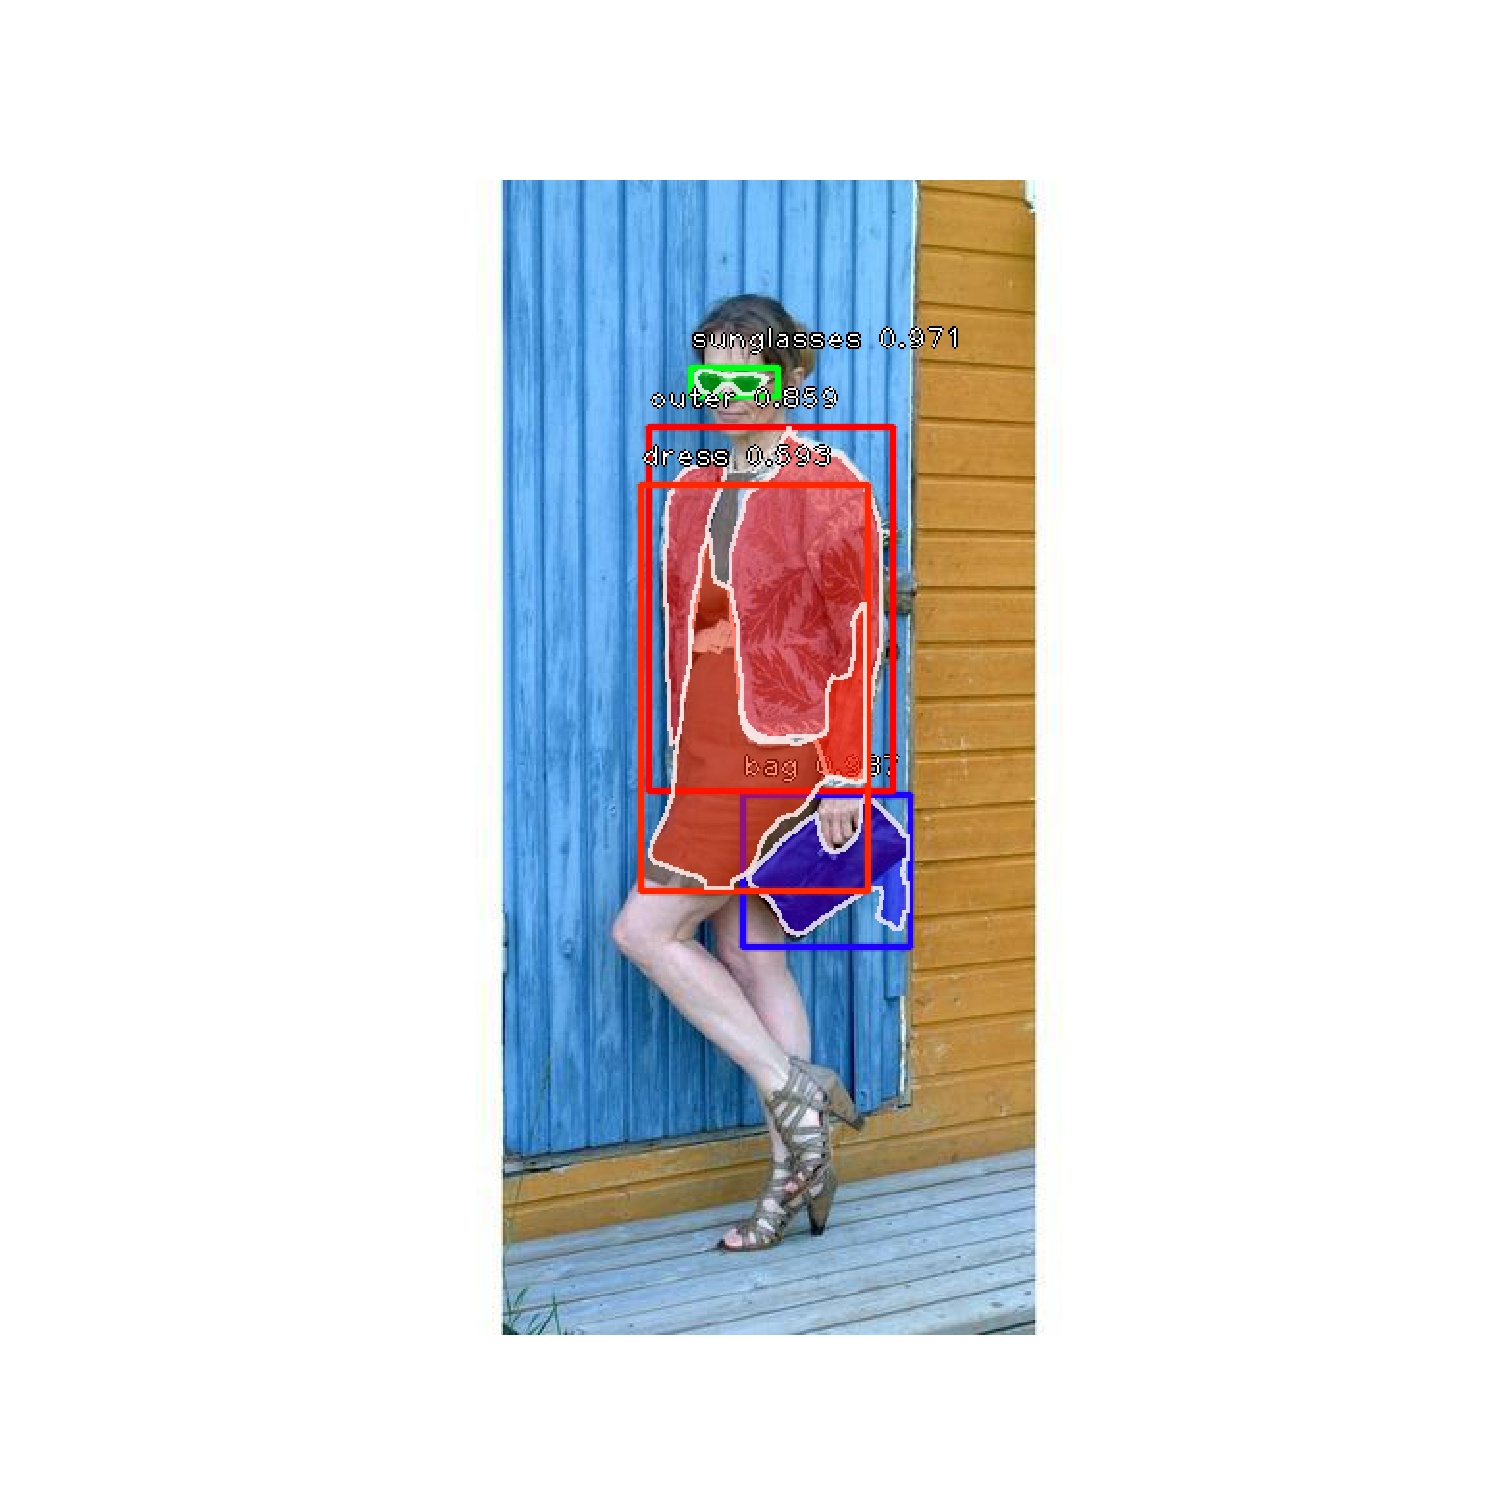
\includegraphics[width=.15\textwidth ,trim=13cm 5cm 13cm 5cm,clip]{figures/processedimages/28fixedindices/0371919} & 
		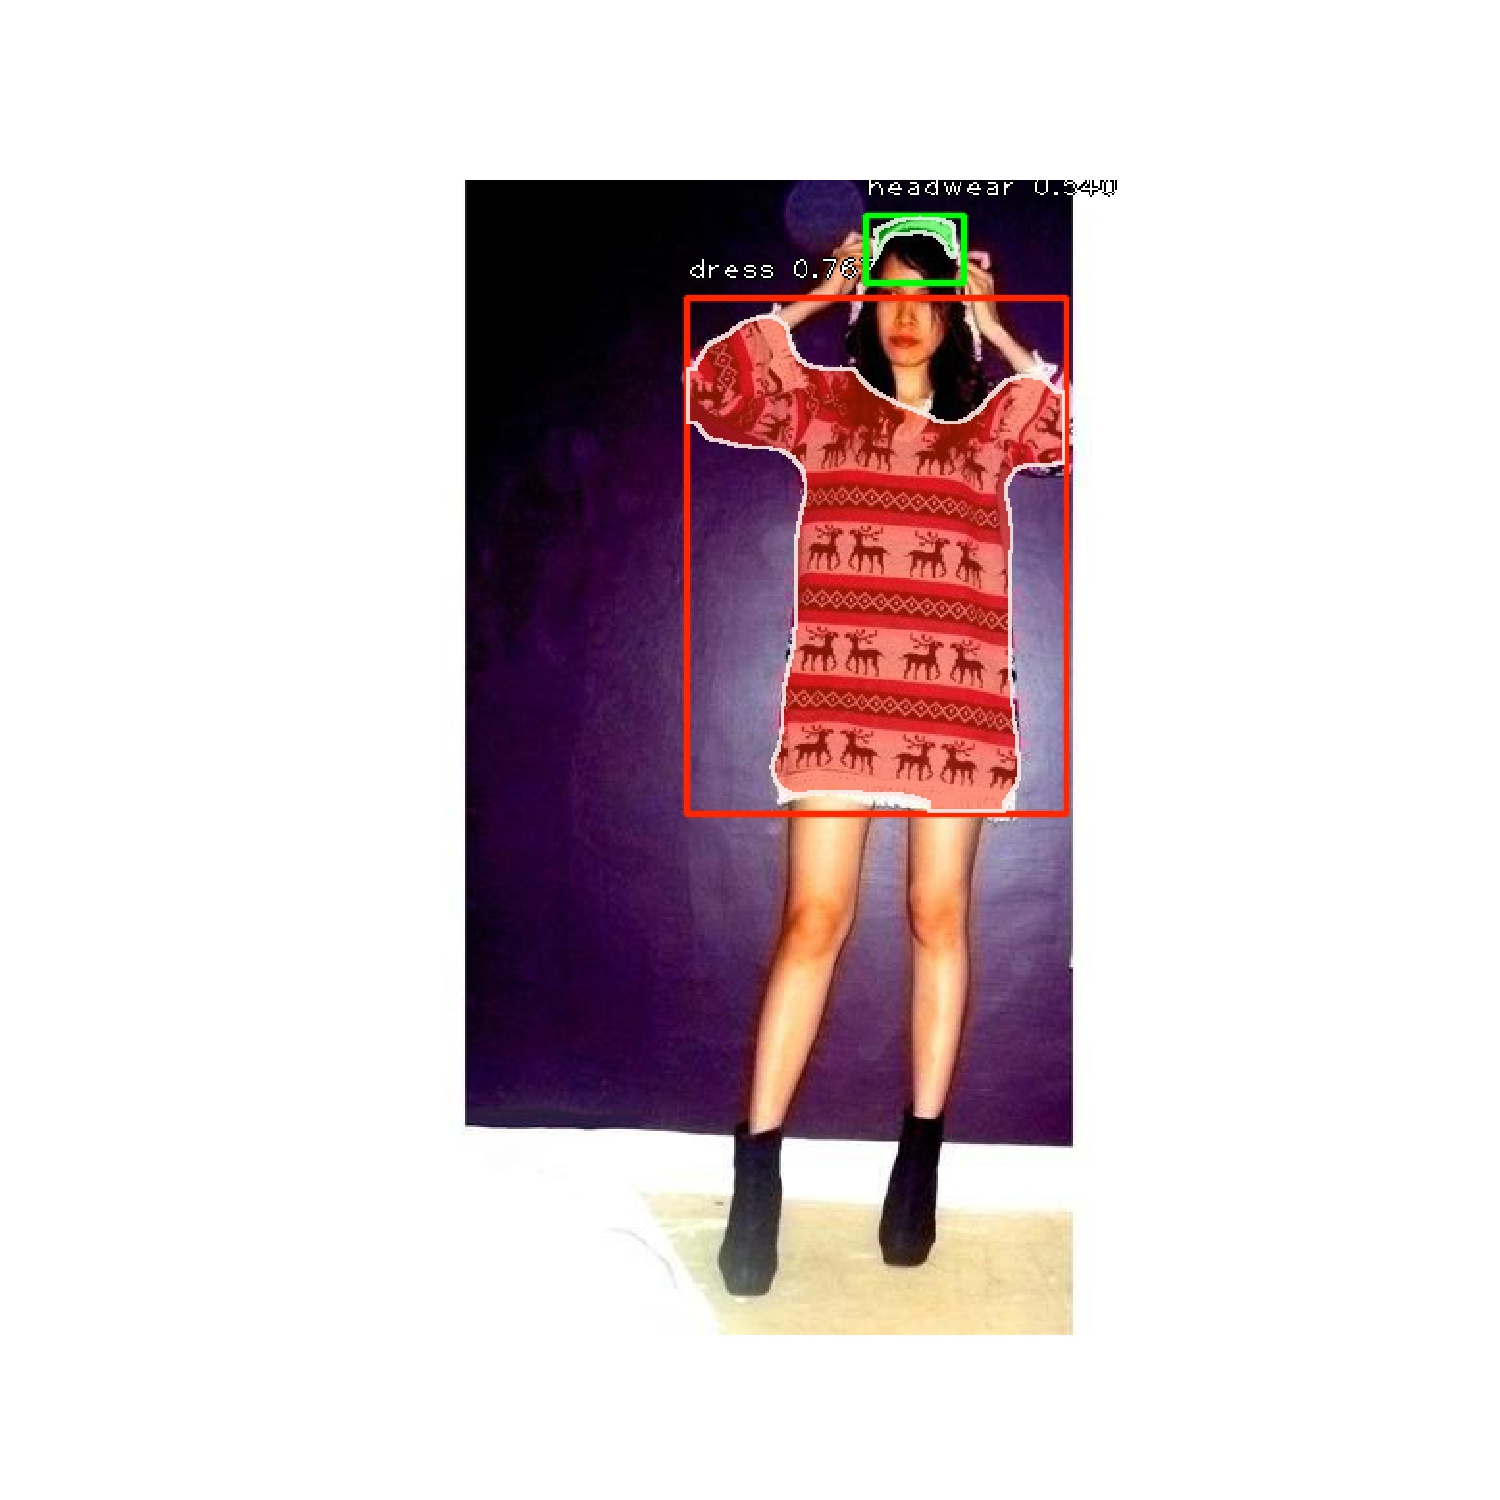
\includegraphics[width=.15\textwidth ,trim=13cm 5cm 13cm 5cm,clip]{figures/processedimages/28fixedindices/0811966} &
		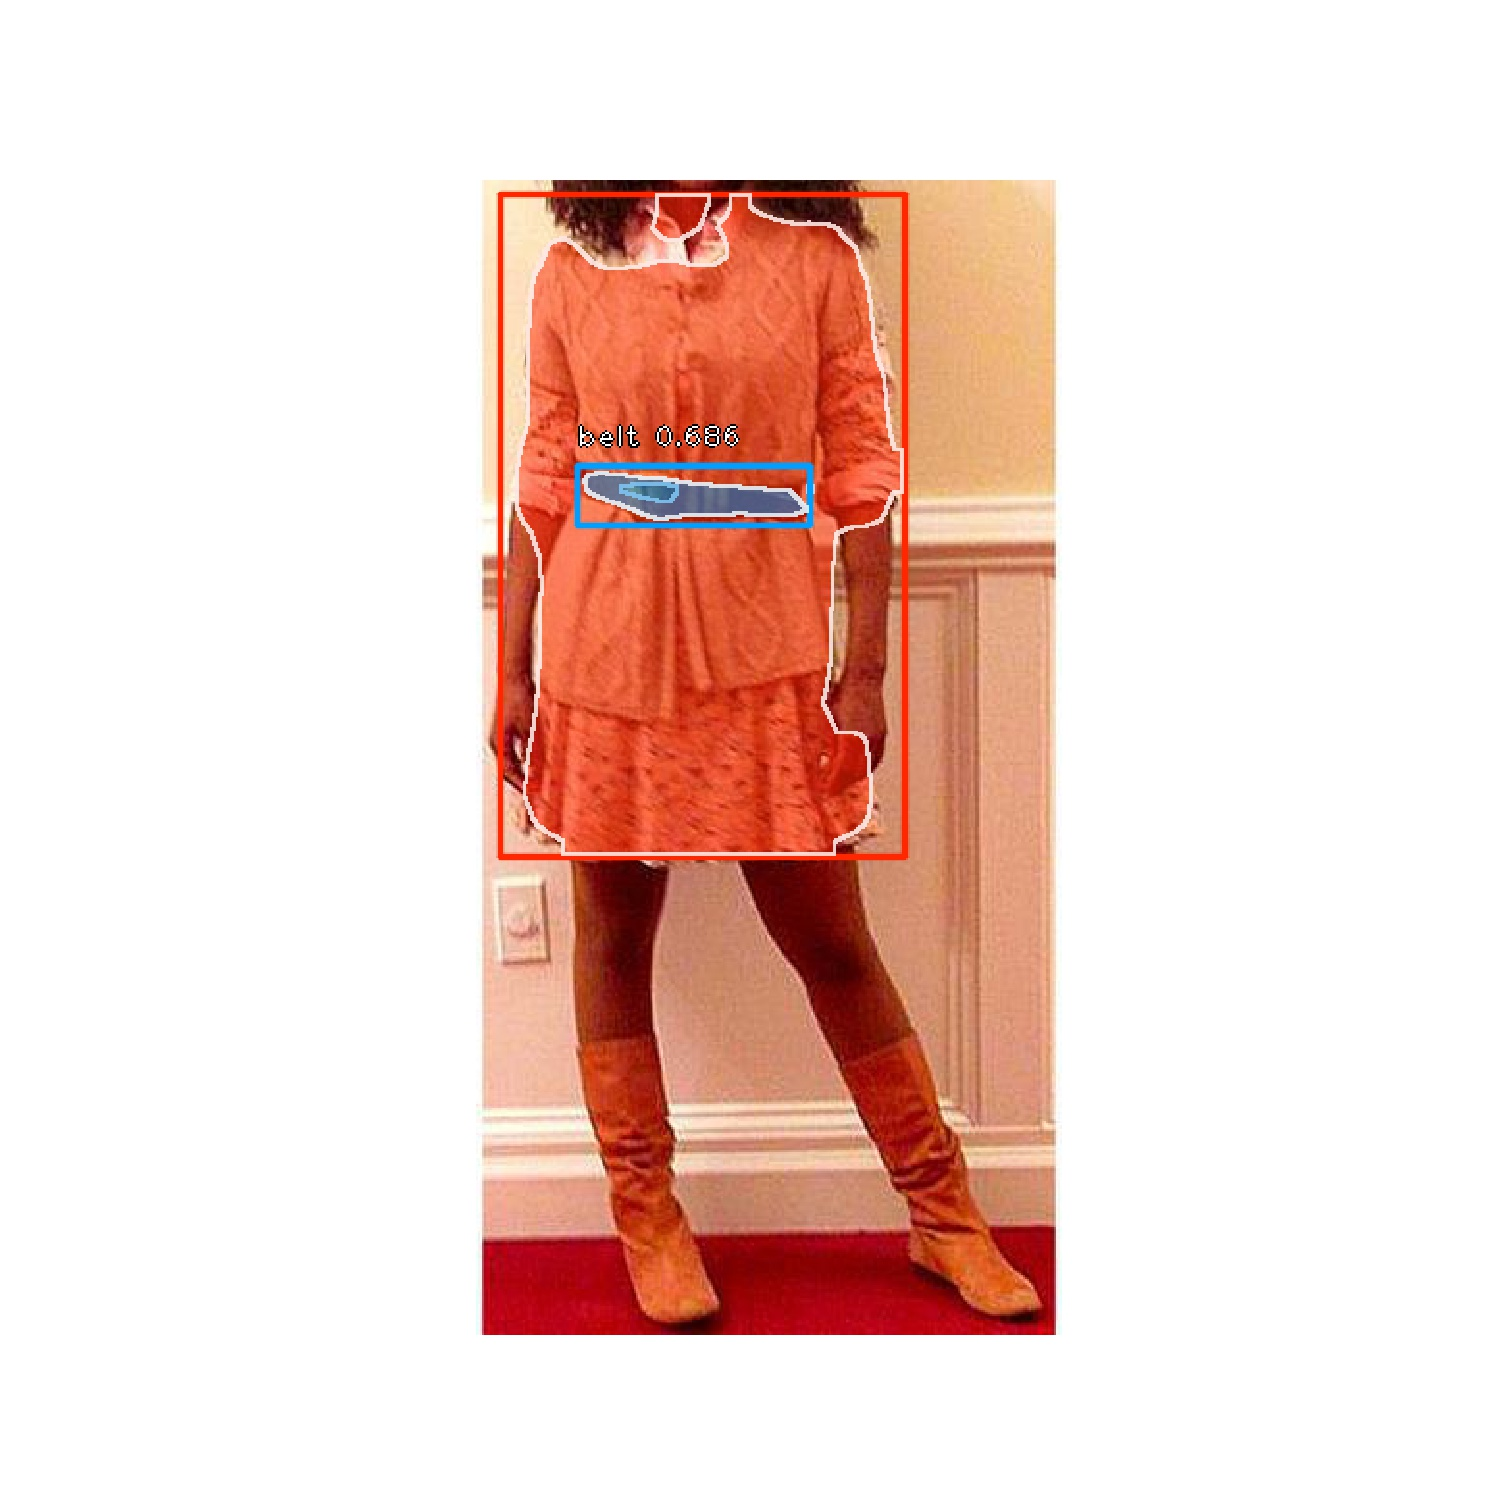
\includegraphics[width=.15\textwidth ,trim=13cm 5cm 13cm 5cm,clip]{figures/processedimages/28fixedindices/0895548} &
		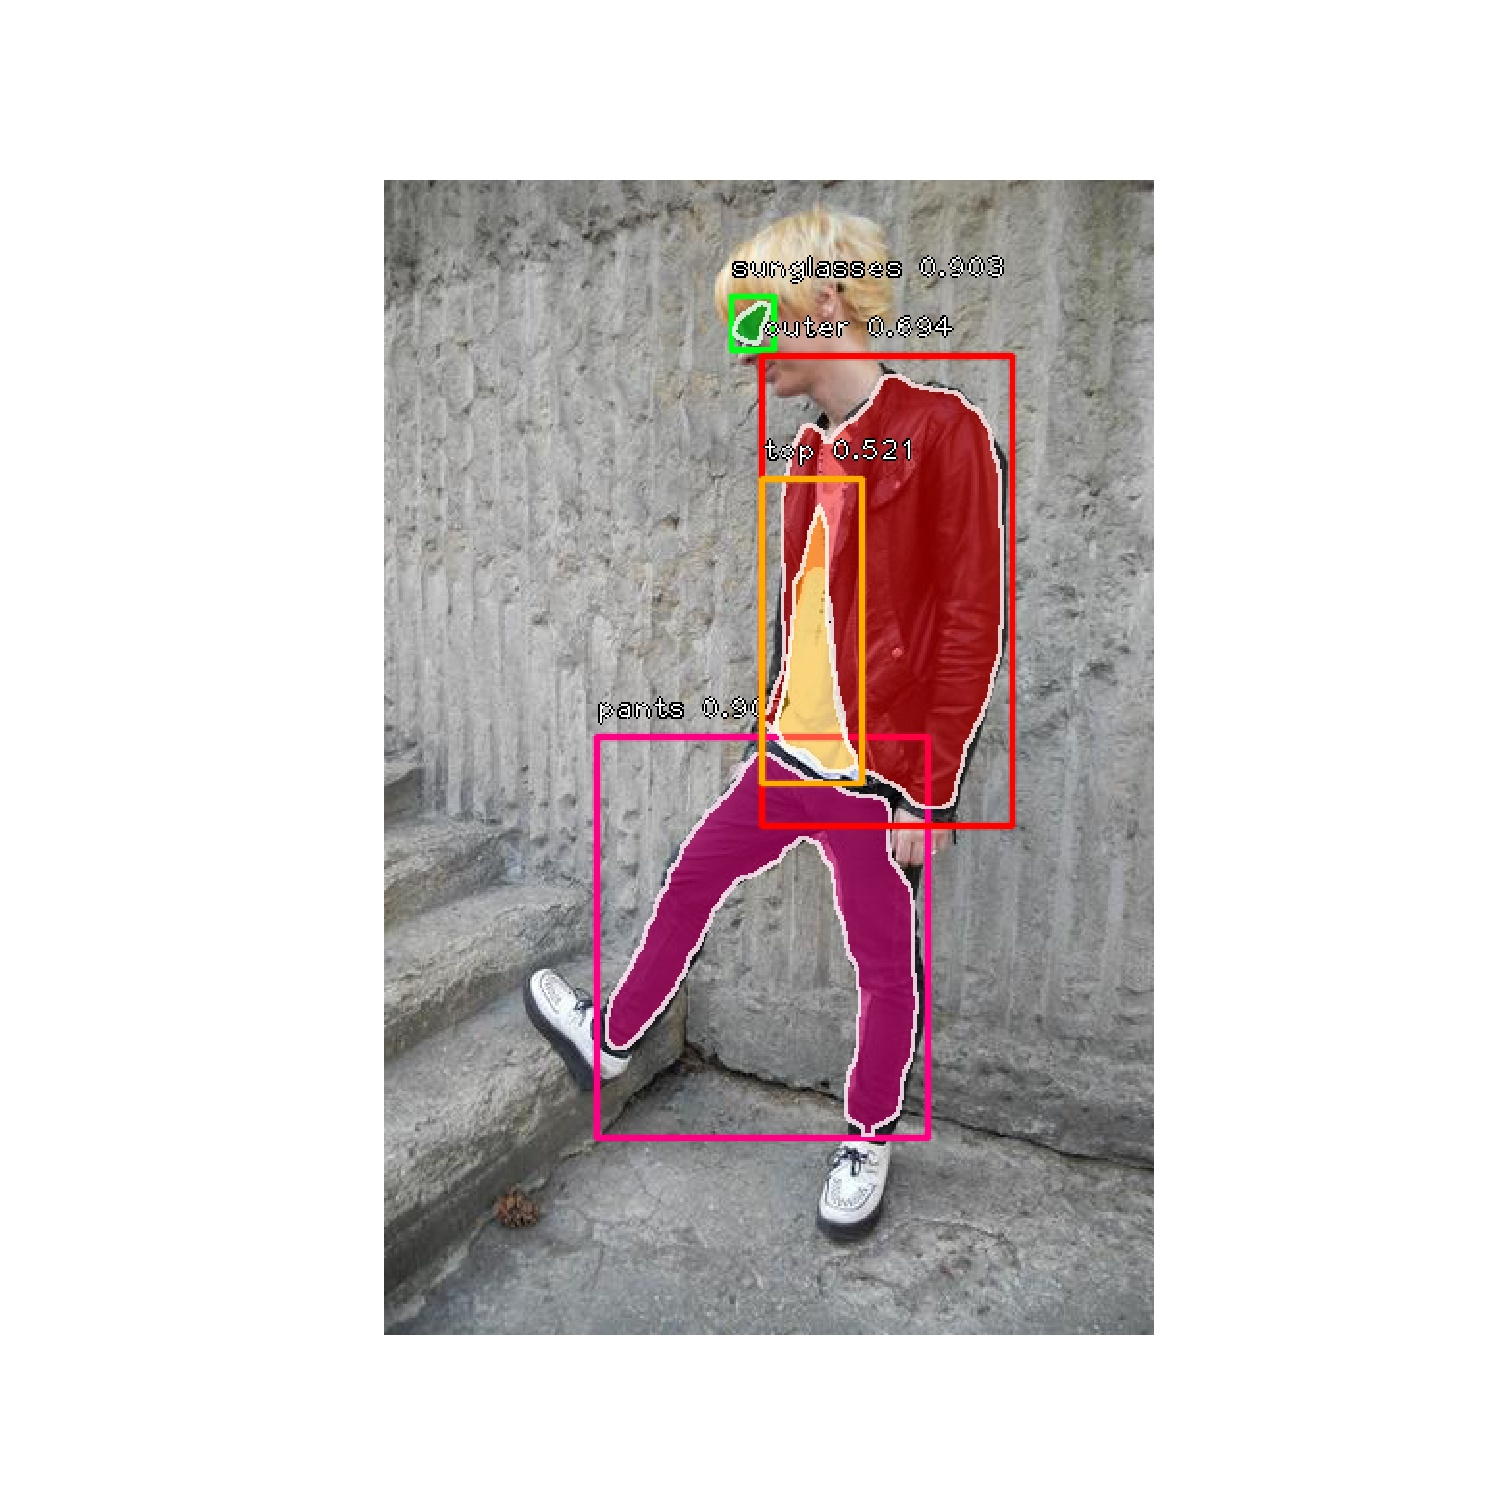
\includegraphics[width=.15\textwidth ,trim=13cm 5cm 13cm 5cm,clip]{figures/processedimages/28fixedindices/1069129} &
		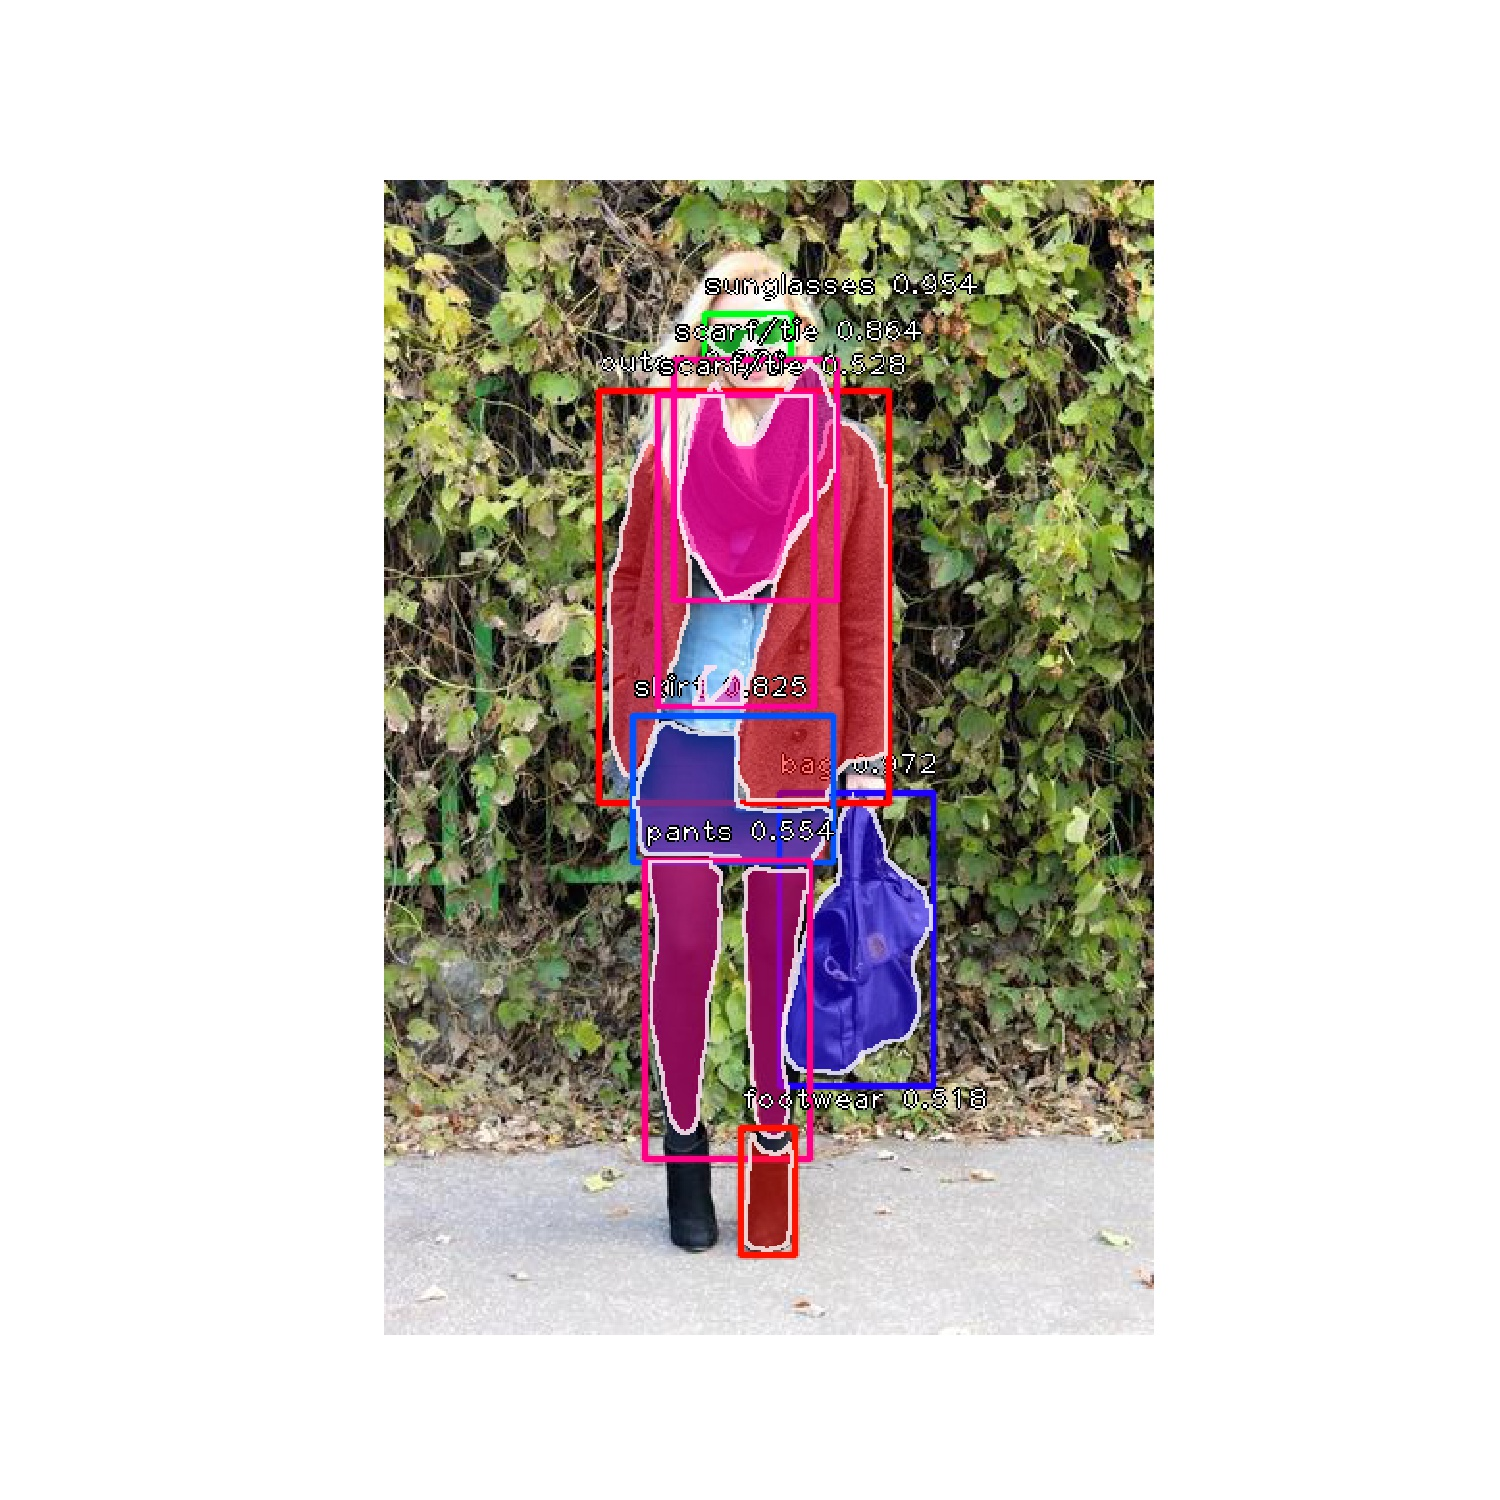
\includegraphics[width=.15\textwidth ,trim=13cm 5cm 13cm 5cm,clip]{figures/processedimages/28fixedindices/1088975} & 
		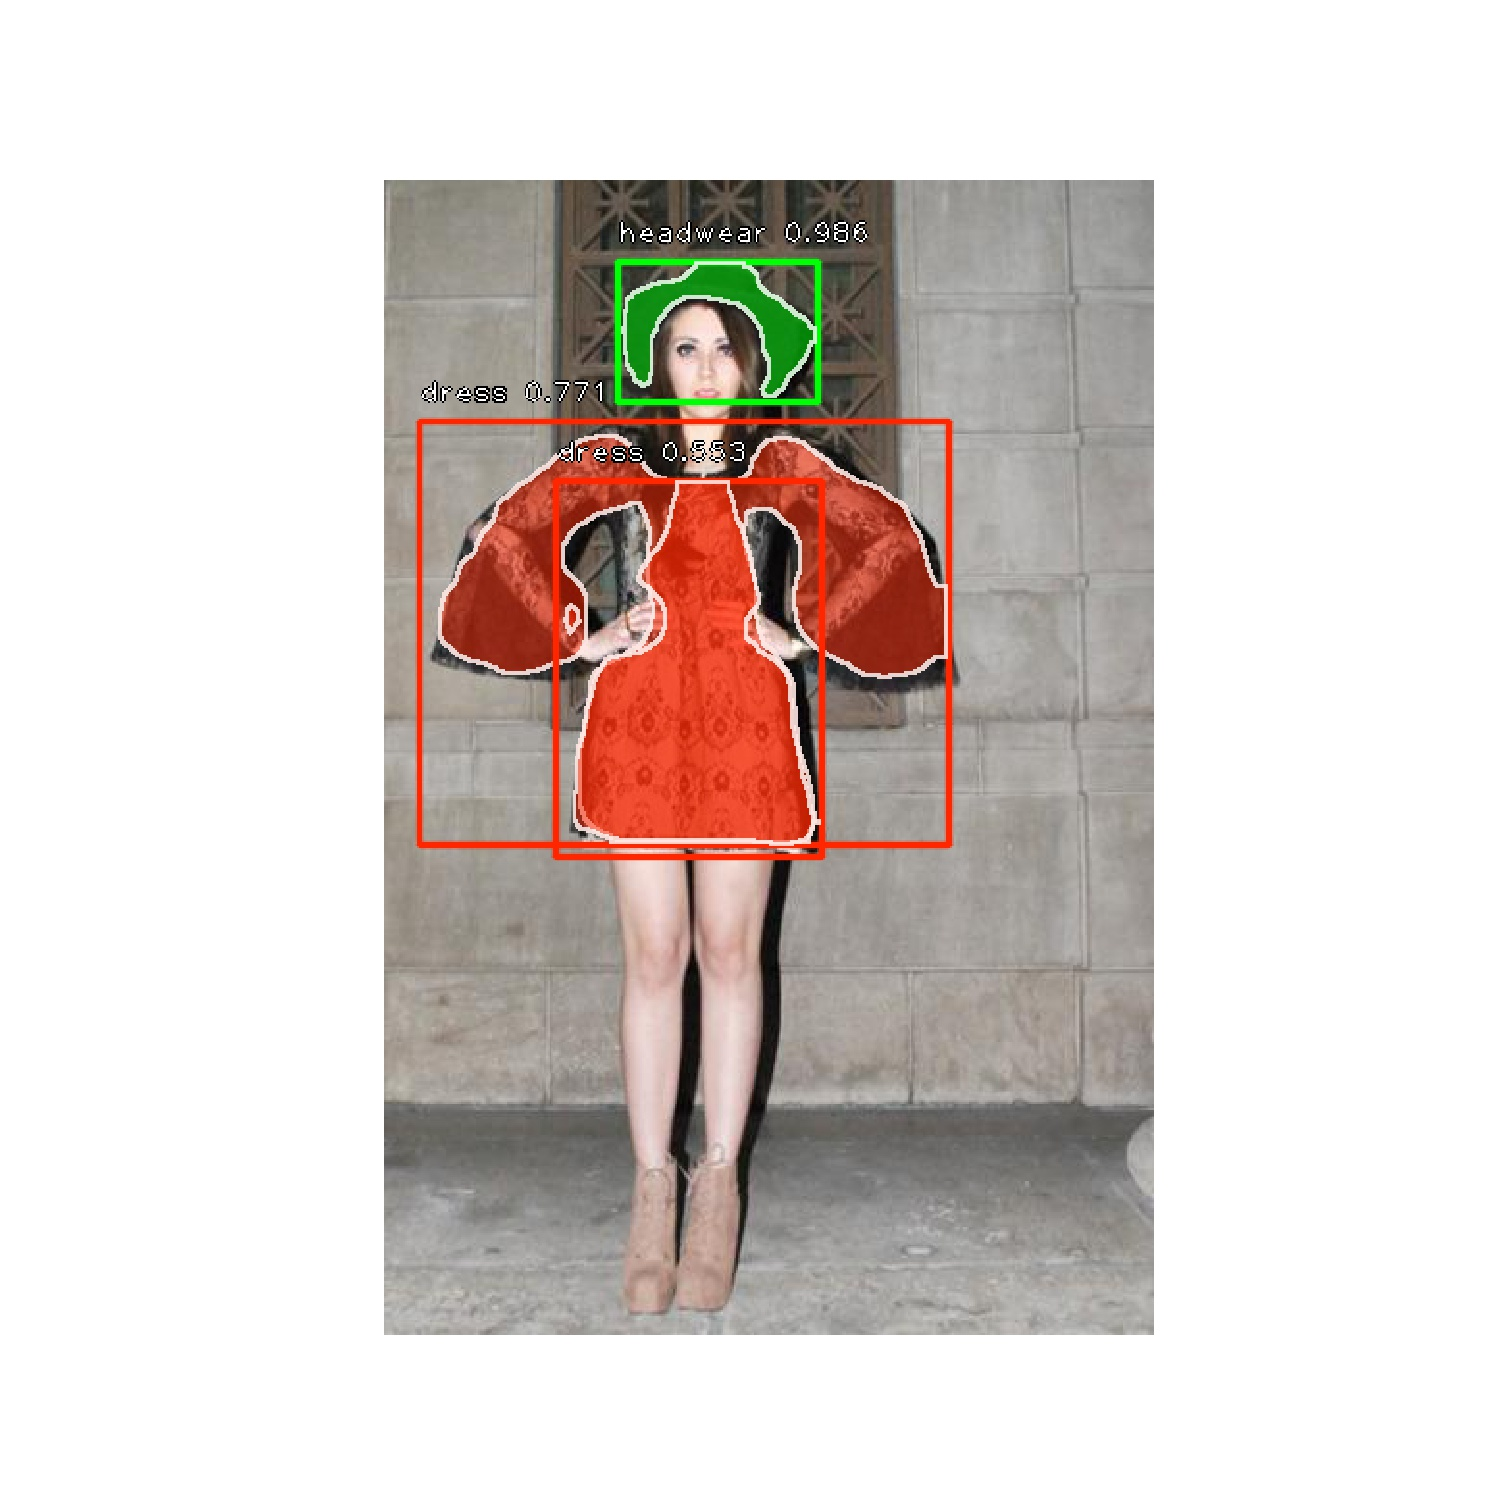
\includegraphics[width=.15\textwidth ,trim=13cm 5cm 13cm 5cm,clip]{figures/processedimages/28fixedindices/1103207}\\
		%\vspace{-5mm}
		%3rd row----------------------------
		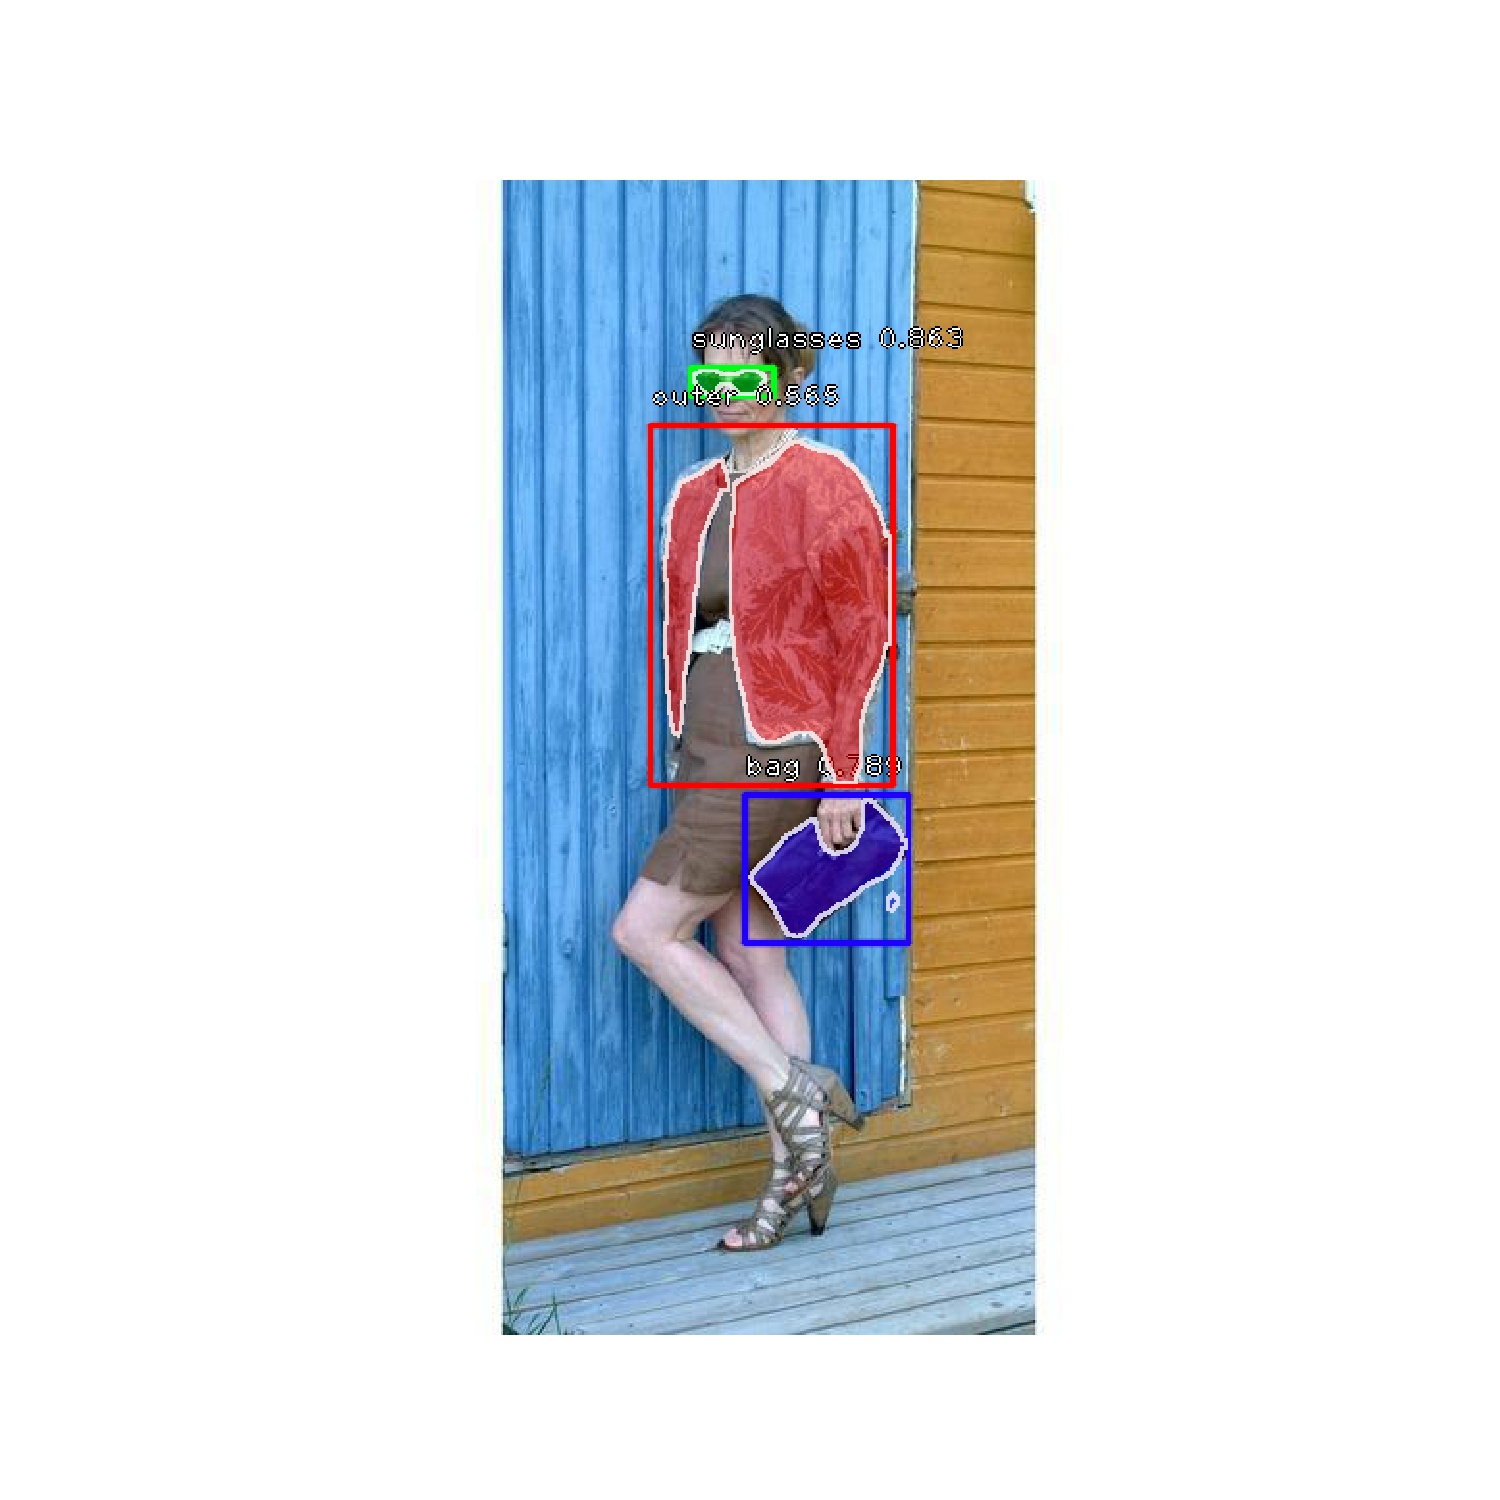
\includegraphics[width=.15\textwidth ,trim=13cm 5cm 13cm 5cm,clip]{figures/processedimages/7afteralmostnewwrongdoubleadded/0371919} & 
		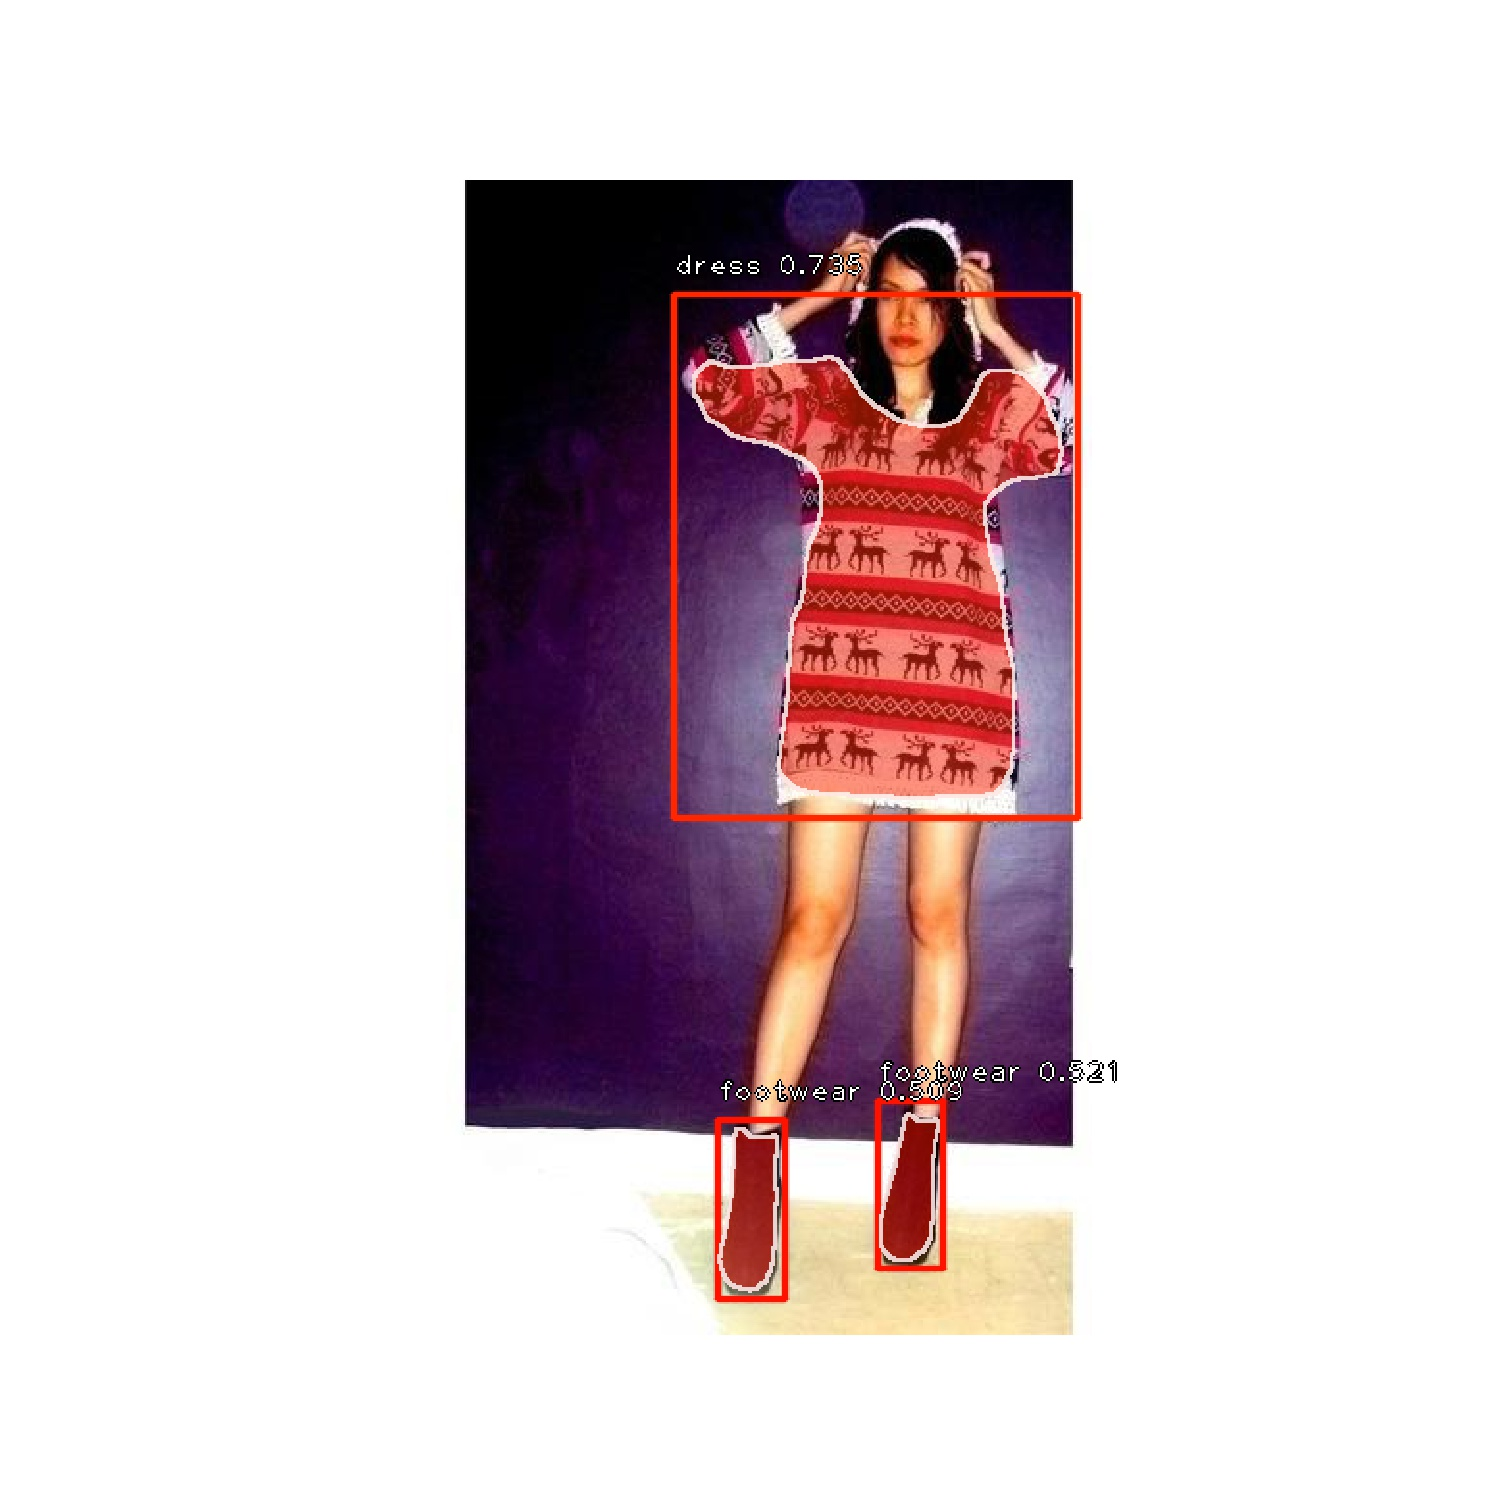
\includegraphics[width=.15\textwidth ,trim=13cm 5cm 13cm 5cm,clip]{figures/processedimages/7afteralmostnewwrongdoubleadded/0811966} &
		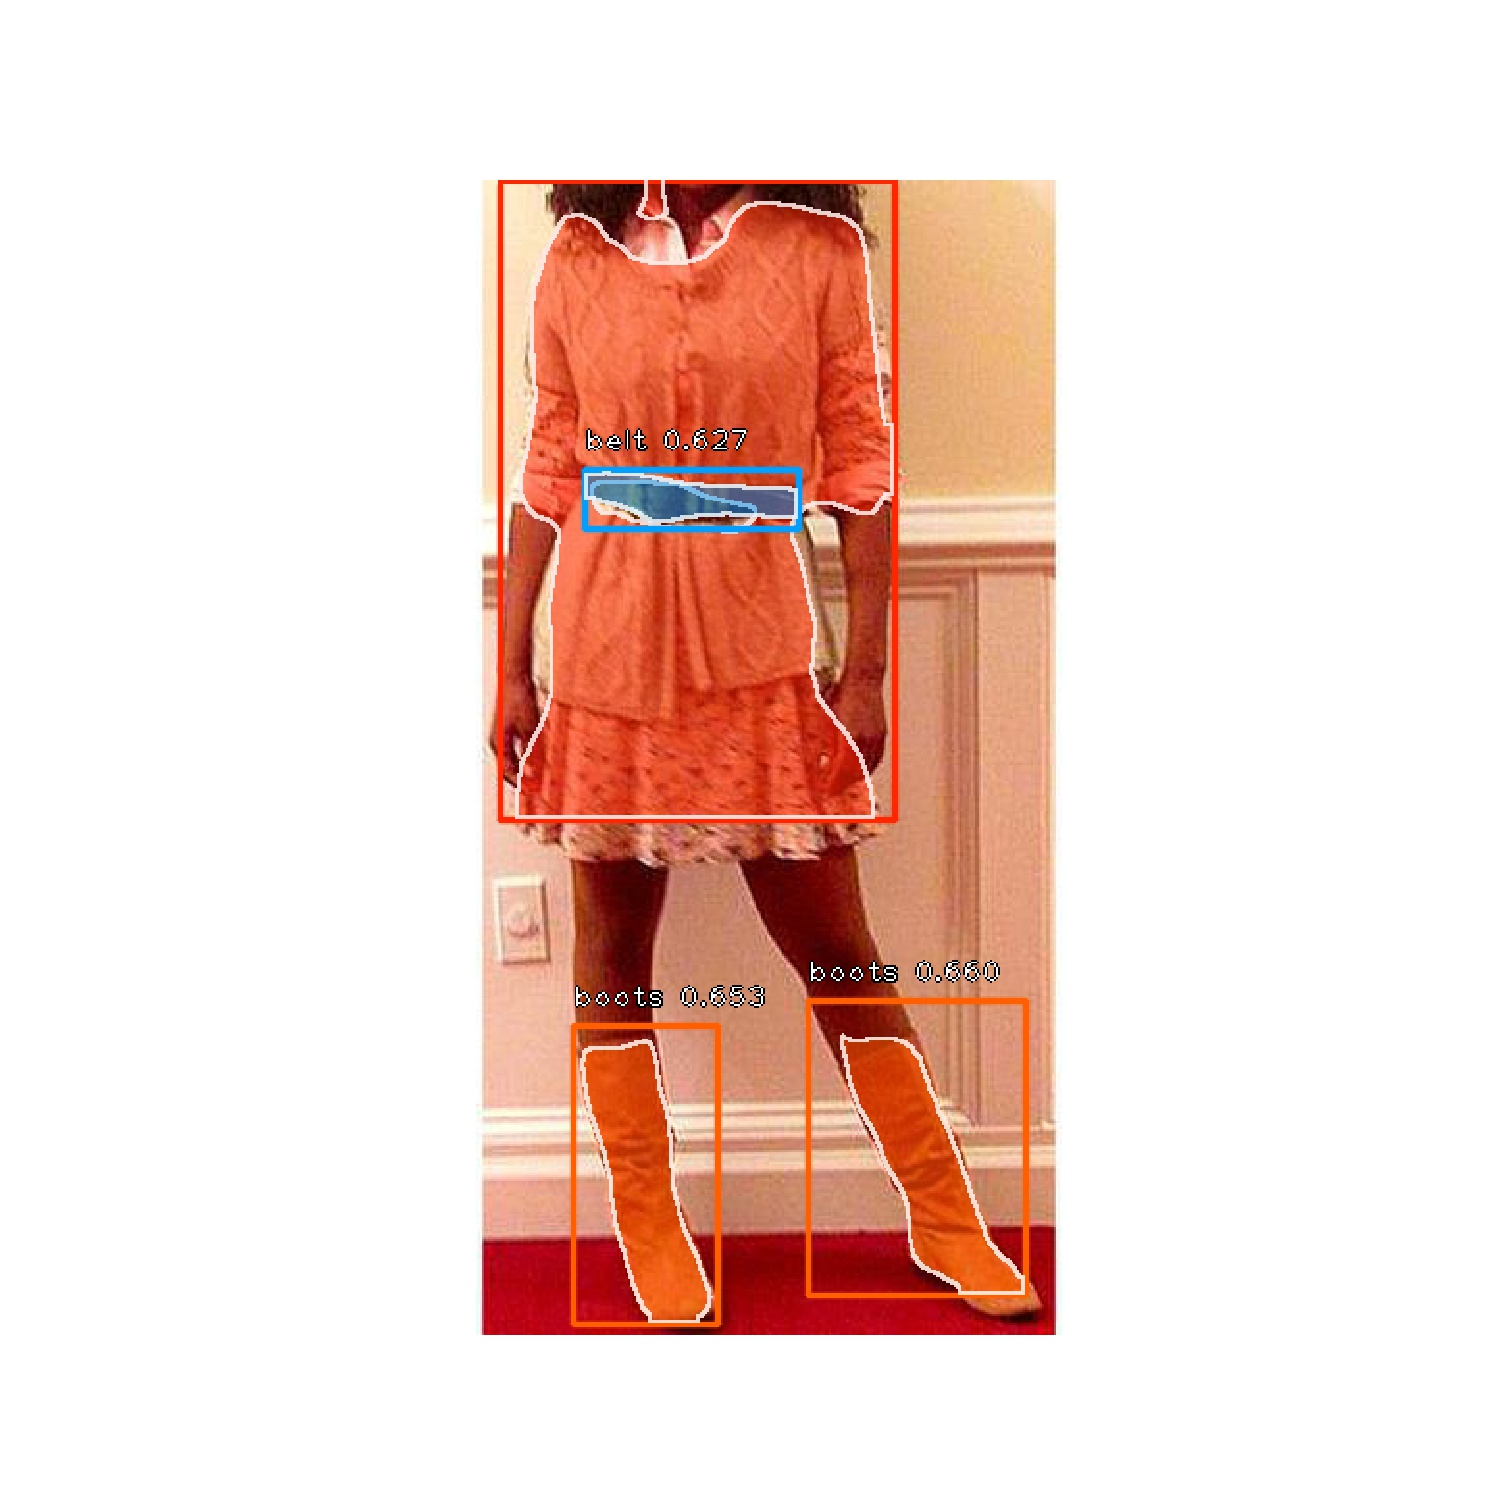
\includegraphics[width=.15\textwidth ,trim=13cm 5cm 13cm 5cm,clip]{figures/processedimages/7afteralmostnewwrongdoubleadded/0895548} &
		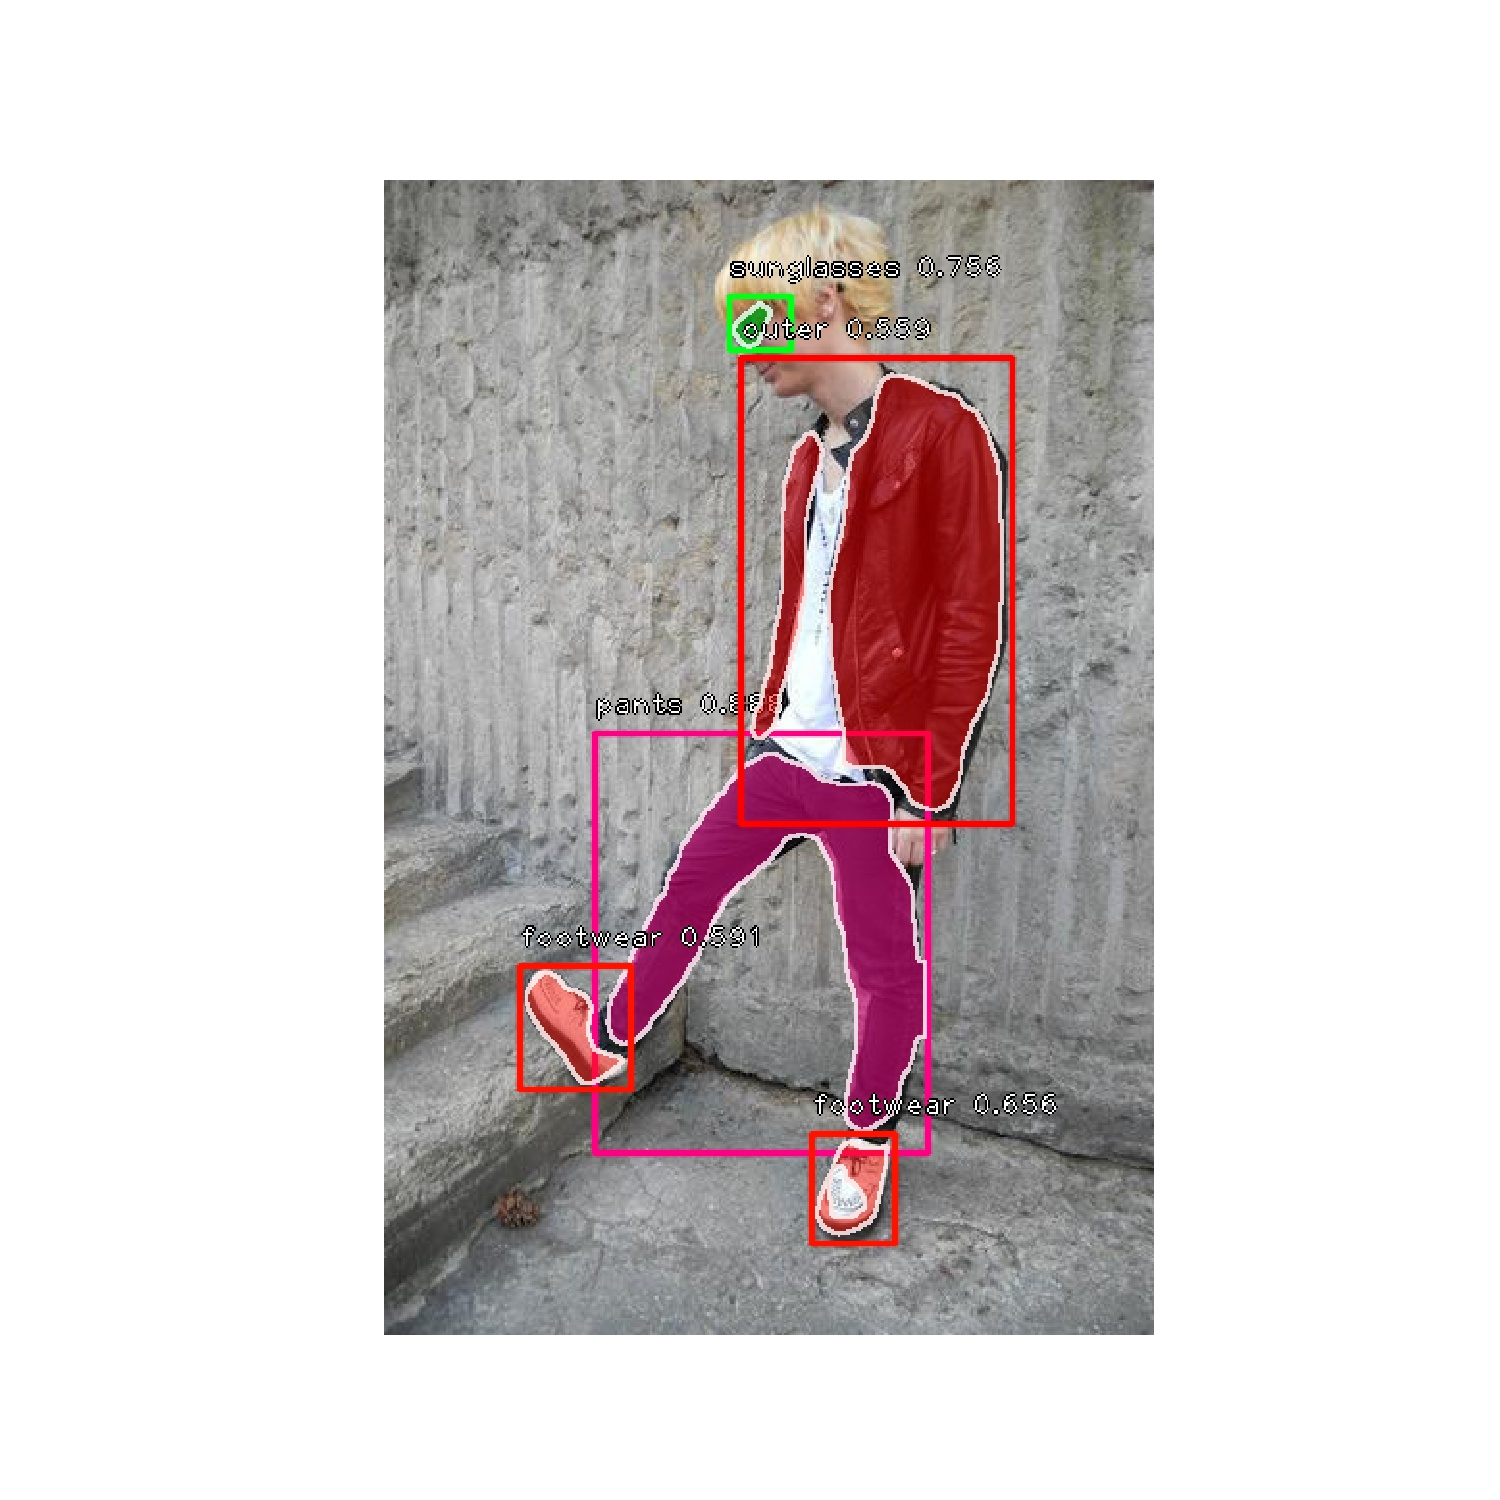
\includegraphics[width=.15\textwidth ,trim=13cm 5cm 13cm 5cm,clip]{figures/processedimages/7afteralmostnewwrongdoubleadded/1069129} &
		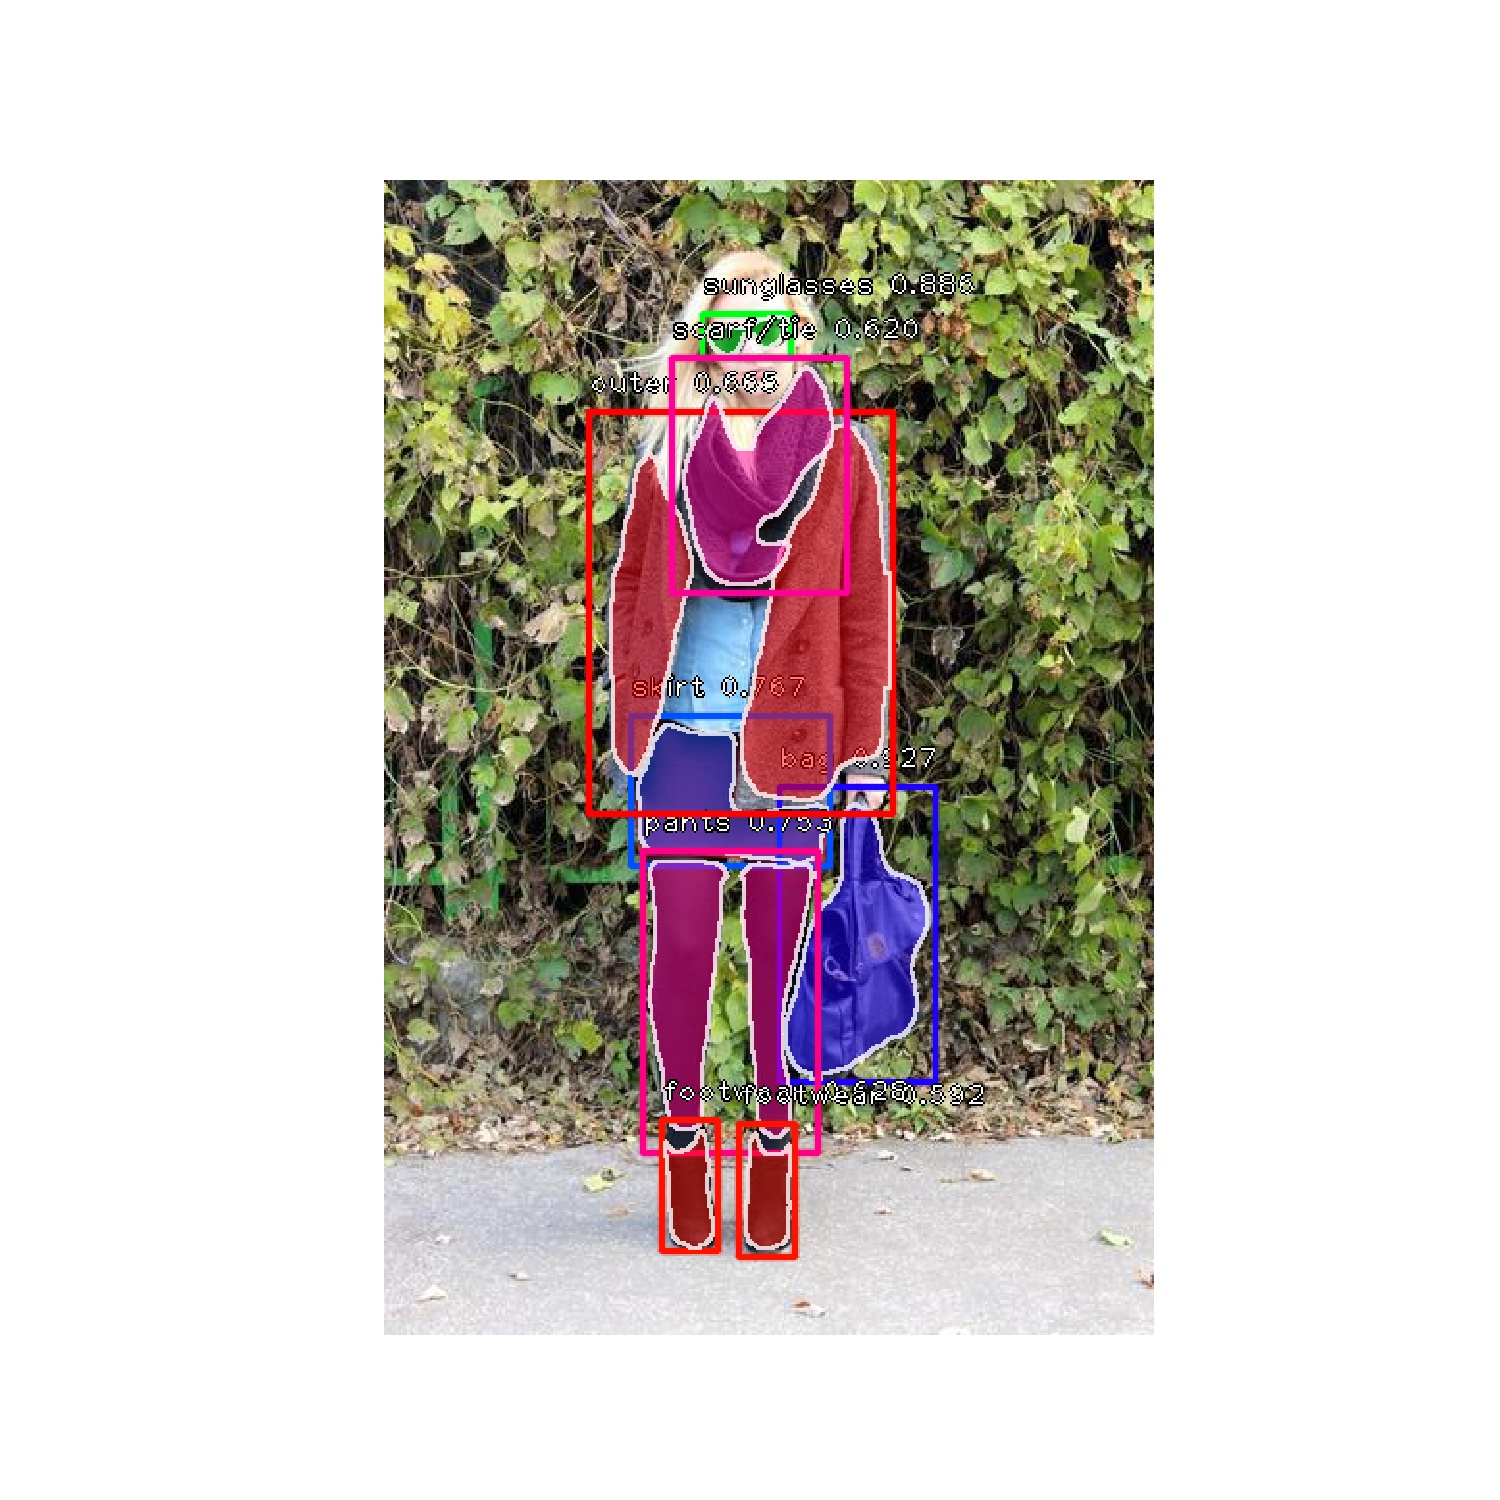
\includegraphics[width=.15\textwidth ,trim=13cm 5cm 13cm 5cm,clip]{figures/processedimages/7afteralmostnewwrongdoubleadded/1088975} & 
		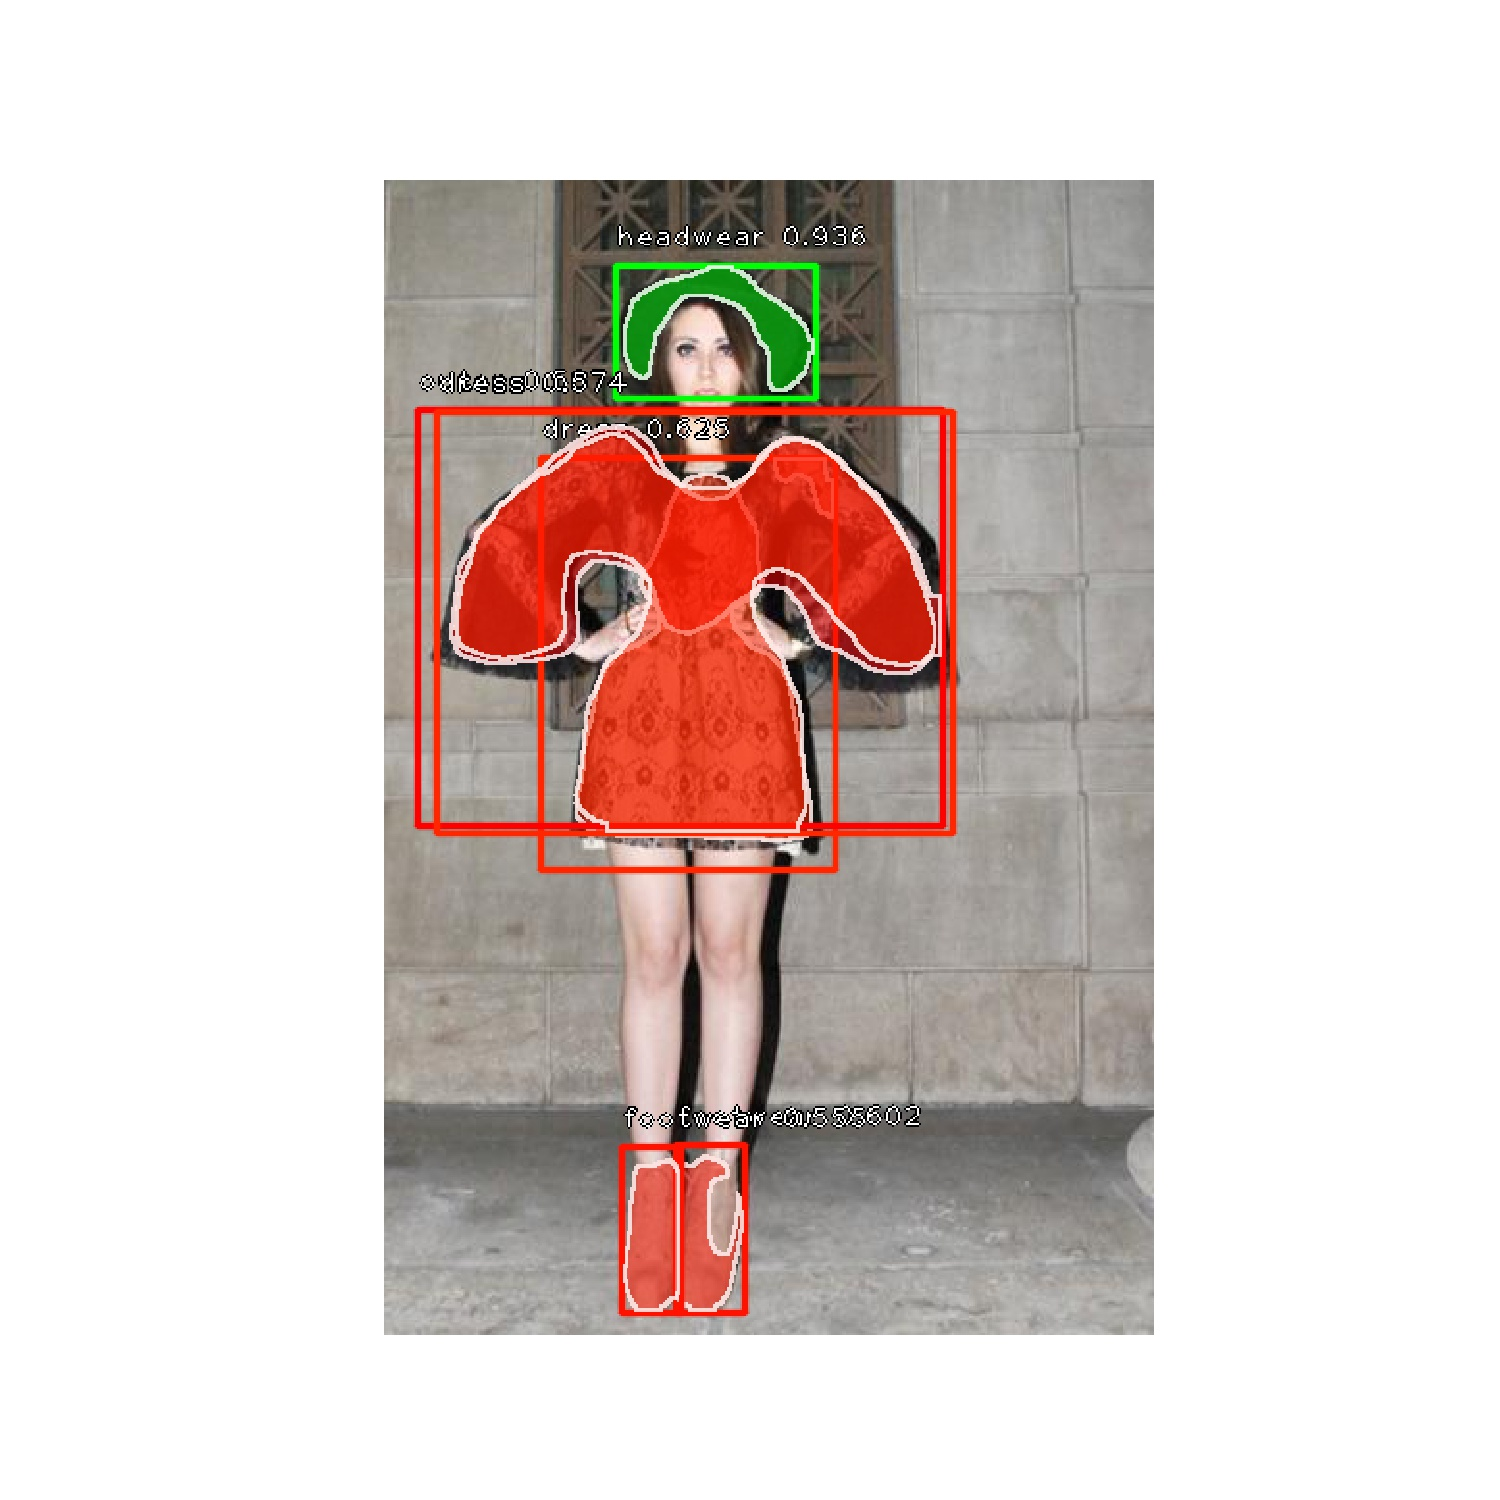
\includegraphics[width=.15\textwidth ,trim=13cm 5cm 13cm 5cm,clip]{figures/processedimages/7afteralmostnewwrongdoubleadded/1103207}\\
		
	\end{tabular}
	\caption{Just like \fref{f:processedimages}, with 6 other images.}
	\label{f:processedimages2} %% label for entire figure
\end{figure}
% --- figure ends --- % 

\subsection{Showing segments instead of full processed image}

This was the first task I was given, as also said on the Abstract. It invoved some knowledge into np arrays. Basically I had to override the function that drew the annotation over the image to make it draw black (or white, whatever, I chose black) outside that particular annotation.
And it would show the results for each segment (annotation) of the image, instead than for the whole image. This has been implemented in the CLI [CLI explained in \sref{s:ds-package}] under an option in the processimage command, which you'll see below in \sref{s:processimage}.

\lstinputlisting[language=Python, breaklines=true, firstline=125, lastline=127]{../maskrcnn-modanet/maskrcnn_modanet/processimages.py}

The key lines above.

\subsection{Processing validation  images}\label{s:processimage}

Processing the image was a pretty standard task, so I started from the file available in the fizyr repo. It basically means: feed the image to the trained neural net and see the result prediction.
I then made it work with a number of options, described in the image below:



You can view or save annotations or images, so there are 4 possible combinations.

\subsection{Viewing custom processed images}

\begin{figure}[H]
	\centering
	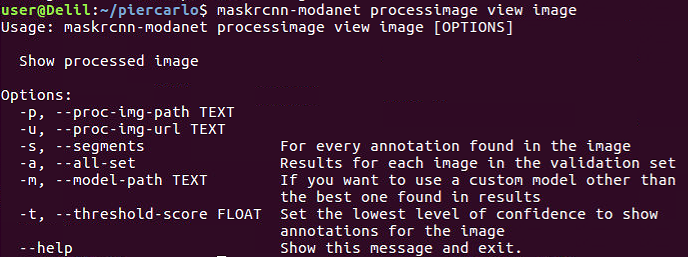
\includegraphics[width=\linewidth]{figures/cli/processimageviewimage}
	\caption{process and view images using a model, a command of the package maskrcnn-modanet}
	\label{f:cli-processimageviewimage}
\end{figure}

\subsubsection{From a path}

The most straightforward way (apart from the --set-all option which is simpler)

\subsubsection{From a URL}

This is interesting and I even showed this as my project for the exam “Telematica".

I first validate that the URL contains a file (and not a text or html).

\lstinputlisting[language=Python, breaklines=true, firstline=41, lastline=61]{../maskrcnn-modanet/maskrcnn_modanet/cli/validators.py}

Then I retrieve the image:

\lstinputlisting[language=Python, breaklines=true, firstline=231, lastline=235]{../maskrcnn-modanet/maskrcnn_modanet/processimages.py}

\subsection{Saving processed images}

\begin{figure}[H]
	\centering
	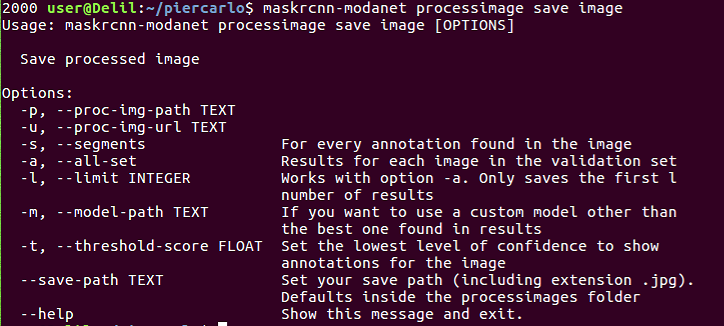
\includegraphics[width=\linewidth]{figures/cli/processimagesaveimage}
	\caption{process and save images using a model, a command of the package maskrcnn-modanet}
	\label{f:cli-processimagesaveimage}
\end{figure}

This is one of the most useful features, especially if you want to see the results of your last training while someone else is training on the same machine, or you are performing another training. And it's always good to never waste processing time in Machine Learning!

The command I use when I finish training is:

\lstinline[language=bash]|maskrcnn-modanet processimage save image -a -l 2000|

-a stands for --set-all and lets me open the whole dataset, -l stands for --limit, so that I only process the first 2000 images, so that I can continue to use the GPU after I finish processing and saving the images.

The program automatically recognizes the best model you have just trained and uses that one, unless you specify one with -m --model-path

And it puts the images into the processedimages/images folder (in results). You can than rename that folder (and recreate it for new trainings).

\subsection{Saving or viewing processed annotations}

This command, I almost never used it. But it was requested that I should have done it, so I did it.

It let's you see the processed annotations. It will probably be useful for future work, when my successor will use those predicted annotations to augment the dataset. (this is just an assumption, I can't predict the future just like a NN can't, for now).

\section{Performance Evaluation}

The performance evaluation is based on several metrics, the most important being AP and AR, explained in \sref{s:trainalg-evalmetrics}. This kind of evaluation is extensively used to easily convert all possible qualitative assumptions in an absolute number, objectionable by only the reliability of that number.

Having said that, the model performing better remains the 28 fixed indices, mainly because of its long time spent training, but qualitative results show that the new model with new annotations is much better at retrieving footwear and shoes. They remain very close though in performance evaluation numbers, as you can check in \sref{s:parameters-and-tests}.

To easily evaluate a model even though training has already been done, I created a command called maskrcnn-modanet evaluate, that takes a parameter -m as the model that you want to evaluate using COCO evauation methods.